\documentclass[10pt,journal]{IEEEtran}

\usepackage{amsmath,amssymb}
\usepackage{booktabs}
\usepackage{tabularx}
\usepackage{graphicx}
\usepackage{float}
\usepackage{placeins}
\usepackage{kotex}
\usepackage{fontspec}
\setmainhangulfont{Noto Serif CJK KR}
\setsanshangulfont{Noto Sans CJK KR}
\usepackage{xcolor}
\usepackage{url}
\usepackage{xspace}
\usepackage{listings}
\usepackage{tikz}
\usetikzlibrary{arrows.meta,positioning,fit,shapes.geometric,calc}
\usepackage[hidelinks]{hyperref}

\definecolor{observed}{RGB}{40,120,90}
\definecolor{derived}{RGB}{40,95,160}
\definecolor{assumed}{RGB}{180,120,35}
\definecolor{blocked}{RGB}{165,55,55}
\definecolor{neutral}{RGB}{70,70,70}

\lstset{basicstyle=\ttfamily\scriptsize,breaklines=true,frame=single,
  columns=fullflexible,showstringspaces=false,captionpos=b,
  abovecaptionskip=5pt,belowcaptionskip=5pt}

\newcolumntype{Y}{>{\raggedright\arraybackslash}X}
\newcolumntype{L}[1]{>{\raggedright\arraybackslash}p{#1}}

\newcommand{\coc}{\textsc{CoC}\xspace}
\newcommand{\uppaal}{\textsc{UPPAAL}\xspace}
\newcommand{\unknown}{미상\xspace}
\newcommand{\preserve}{보존\xspace}
\newcommand{\reset}{재시작\xspace}
\newcommand{\dedup}{중복 제거\xspace}

\renewcommand{\abstractname}{요약}
\renewcommand{\IEEEkeywordsname}{주요어}
\renewcommand{\figurename}{그림}
\renewcommand{\tablename}{표}
\renewcommand{\lstlistingname}{리스팅}
\renewcommand{\refname}{참고문헌}

\renewcommand{\topfraction}{0.95}
\renewcommand{\bottomfraction}{0.90}
\renewcommand{\textfraction}{0.05}
\renewcommand{\floatpagefraction}{0.85}
\renewcommand{\dbltopfraction}{0.95}
\renewcommand{\dblfloatpagefraction}{0.85}
\setcounter{topnumber}{4}
\setcounter{bottomnumber}{3}
\setcounter{totalnumber}{6}
\setcounter{dbltopnumber}{3}

\title{추론 보강형 E2E 자율주행 데이터의 시간·출처 계약 감사: CoC-Nusc와 UPPAAL 기반 분석}

\author{익명 저자}

\begin{document}
\maketitle

\begin{abstract}
사후 생성된 CoC 주석은 추론 보강형 종단간(E2E) 자율주행에 행동 이유를 제공하지만, 반복 주석의 처리, 후보 기한, 응답 연결 및 장면 출처 정책이 없으면 이를 일관된 학습 시퀀스로 해석할 수 없다. 본 논문은 시점이 있는 CoC 주석과 자차 움직임 응답 증거를 출처·계보가 명시된 후보 시간 계약으로 컴파일하고, 기록된 사건열을 재생하는 \uppaal 시간 관찰자로 그 계약을 감사한다. 94개 장면의 단일 이벤트 선별에서 얻은 134개 주석 사건별 후보 계약은 $D=3$~s 분석 설정에서 125+4+5(속도 변화 기준 계약 통과 125개, 이미 만족된 계약 통과 4개, 검토 후보 5개)로 분기되었다. 282개 모델과 1,128개 질의 결과는 레이블에서 직접 설정한 위반 플래그와 기대 판정의 직렬화 회귀 시험으로 한정한다. 반복 정책과 응답 탐지기 설정의 민감도를 함께 검토하고 장면 경계 정책을 오류 차단 시험으로 검사했다. 별도 파서·탐지기를 사용한 비공식 메타데이터 미러 기반 13개 체인 산출물은 구현별 파이프라인 기본 동작 시험일 뿐 공유 계약의 정량 근거로 사용하지 않는다. 이 결과는 새로운 제어의 합성이나 물리적 안전성, CoC 충실도의 독립 증거가 아니라, 학습 전에 저장된 주석의 시간·출처 계약을 점검하는 프로토콜 감사 결과로 해석한다.
\end{abstract}

\begin{IEEEkeywords}
자율주행, E2E 학습, 추론 보강, 모델 체킹, 시간 오토마타, UPPAAL, 데이터 출처, 시간 계약
\end{IEEEkeywords}

\section{서론}
\label{sec:intro}

E2E 자율주행은 카메라, 자차 상태, 경로 조건 등으로부터 미래 궤적 또는 제어 의도를 직접 예측한다. 계획 중심 E2E 연구는 대규모 주행 로그에서 관측 입력과 행동 출력의 관계를 학습하며 \cite{hu2023uniad,jiang2023vad}, 최근의 추론 보강형 E2E/VLA 연구는 여기에 행동 이유를 설명하는 의미 감독을 결합한다. CoC(Chain-of-Causation) 주석은 ``전방 트럭 때문에 감속한다''와 같이 행동 의도와 근거를 함께 제공하므로, 단순 궤적 모방에서 드러나지 않는 학습 신호가 될 수 있다 \cite{sima2024drivelm,tian2024drivevlm,wang2025alpamayo}.

이러한 의미 감독의 근거 정합성, 충실도, 개입과 교란에 대한 반응, 행동 교정은 최근 연구에서 서로 다른 평가 단위로 다루어지고 있다 \cite{xie2025drivebench,zhang2023cat,nvidia2026autolabeler}. 본 논문의 관심은 이 평가들을 대체하는 데 있지 않다. 저장된 시점별 CoC 주석과 자차 움직임을 하나의 학습 시퀀스로 조합할 때, 반복 주석, 후보 기한, 응답 계보, 장면 출처 정책을 어떻게 명시하고 감사할 것인가가 남는 문제이다. 즉, 본 논문은 추론 주석의 내용이 참인지 또는 차량 제어가 안전한지를 판단하지 않고, 선택된 정책 아래 주석과 자차 움직임 응답 증거가 시간·출처 계약을 이루는지를 다룬다.

\begin{figure*}[t]
\centering
\resizebox{0.95\textwidth}{!}{%
\begin{tikzpicture}[
  main/.style={draw, rounded corners=2pt, align=center, minimum height=12mm,
    text width=3.05cm, font=\footnotesize},
  stage/.style={draw, rounded corners=2pt, align=center, minimum height=8mm,
    text width=3.45cm, font=\scriptsize, fill=black!3},
  data/.style={main, fill=observed!10},
  reason/.style={main, fill=derived!10},
  contract/.style={main, fill=assumed!12},
  route/.style={main, fill=neutral!8},
  flow/.style={-{Latex[length=2mm]}, thick, draw=black!80},
  guide/.style={-{Latex[length=1.5mm]}, thin, dashed, draw=black!45}
]

% Main narrative.
\node[data] (log) at (0,0) {Driving video\\ego trajectory};
\node[reason] (llm) at (4.0,0) {VLM/LLM\\CoC reasoning};
\node[contract] (obl) at (8.0,0) {Abstract intent\\timed obligation};
\node[contract] (monitor) at (12.0,0) {UPPAAL\\episode observer};
\node[route] (route) at (16.0,0) {감사 라우팅\\약한 유지 후보ㆍ검토 후보\\출처 불충분};

\draw[flow] (log) -- coordinate[midway] (m1) (llm);
\draw[flow] (llm) -- coordinate[midway] (m2) (obl);
\draw[flow] (obl) -- coordinate[midway] (m3) (monitor);
\draw[flow] (monitor) -- coordinate[midway] (m4) (route);

% Process interpretation row.
\node[stage] (s1) at (2.0,-1.55) {Auto-labeling from\\recorded trajectory};
\node[stage] (s2) at (6.0,-1.55) {Intent/hazard parsing\\quality gate};
\node[stage] (s3) at (10.0,-1.55) {Deadline/repeat semantics\\response evidence};
\node[stage] (s4) at (14.0,-1.55) {Verdict report\\with counterexample provenance};

\draw[guide] (m1) -- (s1.north);
\draw[guide] (m2) -- (s2.north);
\draw[guide] (m3) -- (s3.north);
\draw[guide] (m4) -- (s4.north);

% Takeaway.
\node[draw=assumed, rounded corners=2pt, align=center, font=\footnotesize,
  fill=assumed!8, text width=14.0cm] (key) at (8.0,-3.0)
  {Key point: reasoning is a learnable semantic signal, but trigger, repeat, deadline, and response matching must be defined before it becomes a verifiable timed contract.};

\end{tikzpicture}%
}

\caption{추론 보강형 E2E 주행 데이터를 시간·출처 계약 감사 대상으로 변환하는 절차. 영상과 자차 궤적에서 생성된 CoC 추론은 학습 가능한 의미 신호이지만, 시작 사건, 반복, 후보 기한, 응답 매칭과 출처 정책을 정의해야 감사 가능한 후보 시간 의무가 된다.}
\label{fig:overview-pipeline}
\end{figure*}

그림~\ref{fig:overview-pipeline}은 이 감사의 흐름을 요약한다. 주행 영상과 자차 궤적은 관측 가능한 원천 증거이고, VLM/LLM 기반 CoC는 이 기록에 사후적으로 결합된 판단 이유와 행동 의도를 제공한다. 본 논문은 품질 관문을 통과한 CoC 주석 사건을 추상 의도와 후보 시간 의무로 변환하고, \uppaal 관찰자로 시작·반복 사건, 후보 기한, 자차 움직임 응답 증거와 출처 정책을 함께 검사한다. 산출물은 물리적 안전성의 판정이 아니라 계약 통과, 정책·민감도 의존 검토 후보, 출처 불충분 사례 및 검사기 시험용 합성 변이를 구분하는 감사 기록이다.

동기 사례인 `CoC-Nusc'의 \texttt{scene-0001}에는 전방 트럭과 공사 구간을 이유로 한 감사 수용 \textsc{Decelerate} CoC 주석 사건이 2.5초에 발생하고, 유사한 감속 주석이 3.5초와 4.8초에 반복된다. 기본 탐지기가 자차 속도 궤적에서 찾은 지속적 속도 감소 시작은 4.6597초이다. \preserve 정책에서는 2.5초의 사건이 대기 중인 후보 시간 의무를 열고 반복 주석은 시계를 다시 시작하지 않으므로, 2초 후보 기한에서는 검토 후보가 되고 3초에서는 계약을 통과한다. 반대로 3.5초의 반복 주석에 \reset 정책을 적용하면 같은 자차 움직임 응답 증거가 1.1597초 뒤에 발생한 것으로 계산되어 2초 계약도 통과할 수 있다. 이 차이는 정책을 명시하지 않을 때 동일 기록의 감사 판정이 달라짐을 보이는 민감도 사례이지, 해당 장면을 안전하지 않은 사례로 분류하는 근거는 아니다.

CoC 주석 사건은 액추에이터 명령이 아니다. CoC-Nusc의 CoC는 기록된 자차 궤적에서 메타 행동을 추출한 뒤 영상 및 궤적과 함께 생성된 trajectory-conditioned 회고적 주석이므로, 같은 궤적과의 일치는 독립적인 인과 검증이 아니다. 본 논문에서 각 주석 사건은 추상 제어 의도와 후보 시간 의무의 입력을 제공하며, 관측 가능한 반응은 자차 속도·궤적에서 도출한 자차 움직임 응답 증거이다. 따라서 이 감사는 CoC의 일반적 충실도나 차량 안전성을 증명하지 않고, 선택한 시간·출처 정책 아래 저장된 주석과 응답 증거의 조합이 일관적인지를 검사한다.

이 사례로부터 본 논문은 다음 연구 질문을 다룬다.
\begin{enumerate}
    \item \textbf{RQ1 변환 타당성:} 시점이 있는 CoC 주석과 자차 움직임을 증거 수준이 명시된 시간 관찰자 네트워크로 변환할 수 있는가?
    \item \textbf{RQ2 판정 민감도와 검토 후보:} 반복 의미론, 후보 기한과 응답 탐지기 설정이 동일 기록의 감사 판정과 검토 우선순위를 어떻게 바꾸는가?
    \item \textbf{RQ3 출처와 장기 에피소드:} 장면 연속성 증거와 경계 정책은 어떤 주석을 장기 학습 시퀀스로 묶을 수 있는지 어떻게 제한하는가?
    \item \textbf{RQ4 정형화의 부가가치:} 결정적 타임스탬프 스크립트와 비교할 때 UPPAAL 관찰자 네트워크는 어떤 명세, 조합과 반례 추적상의 부가가치를 제공하는가?
\end{enumerate}

각 연구 질문에 대한 증거 범위가 제한된 기여는 다음과 같다.
\begin{enumerate}
    \item \textbf{RQ1:} CoC 주석 사건, 자차 움직임 응답 증거 및 출처·계보를 시간 관찰자 네트워크로 컴파일하고, 알려진 합성 변이에 대한 기대 판정 일치로 입력 사건과 관찰자 질의의 표현 범위를 확인한다.
    \item \textbf{RQ2:} 적용 가능 계약 집합에서 반복 정책, 후보 기한 및 응답 탐지기 설정에 따른 감사 판정의 변화를 유형화하여, 검토 후보가 정책과 민감도에 의존함을 기록한다.
    \item \textbf{RQ3:} 장면별 시간·자세 초기화의 오류 차단 시험을 통해 출처 증거가 없는 장면 이월을 차단하고, 연결 적격성과 연결 후 계약 감사를 분리하는 정책을 제시한다. 별도 파서·탐지기의 체인 산출물은 구현 기본 동작 시험으로만 보고한다.
    \item \textbf{RQ4:} 구현별 모델군에서 의무 생명주기, 반복·경계 정책, 변이 오라클 및 교착 질의를 검토 가능한 명세로 표현하는 역할을 명확히 한다. 보존된 집계 산출물의 13/13 일치는 독립 구현 재현성 주장이 아니라 기록된 일치값으로만 다룬다.
\end{enumerate}

본 논문의 주장 범위는 프로토콜 수준 시간·출처 계약 감사로 제한된다. 검사 대상은 CoC 주석 사건, 후보 기한, 자차 움직임 응답 증거 및 출처 정책의 정합성이다. 상대 객체 상태, 액추에이터 명령, 차량 동역학 및 폐루프 결과가 없으므로 충돌 회피, 안전거리 또는 배포 가능한 제어 안전성은 결론으로 판정하지 않는다. 이 감사는 더 강한 폐루프 및 물리 안전성 평가 이전에 학습 자료의 해석 계약을 분리해 점검하는 단계이다.

\begin{table}[t]
\centering
\caption{본 논문에서 사용하는 주요 용어.}
\label{tab:terminology}
\footnotesize
\begin{tabularx}{\columnwidth}{L{0.35\columnwidth}Y}
\toprule
Term & Meaning \\
\midrule
CoC annotation event & A timestamped retrospective CoC annotation, not an actuator command \\
Audit-accepted event & An input accepted by machine quality gates, not a human-gold or causal-truth label \\
Parsed intent & Abstract action category such as \textsc{Decelerate}, \textsc{Stop}, or \textsc{Yield} \\
Candidate audit obligation & A researcher-specified, time-bounded annotation--response-evidence contract \\
Ego-motion response evidence & Evidence derived from speed/trajectory, not an actuator command \\
Episode & Ordered annotation and response-evidence sequence within one local clip or provenance-supported chain \\
Scene boundary & Boundary that closes a pending obligation without inter-scene continuity evidence \\
Mutation oracle & Synthetic condition used to check observer verdicts, not an estimate of real fault prevalence \\
\bottomrule
\end{tabularx}
\end{table}

표~\ref{tab:terminology}의 용어 구분은 본 논문의 주장 범위를 제한하기 위해 필요하다. 특히 CoC 주석 사건, 후보 시간 의무, 자차 움직임 응답 증거를 분리해야 CoC 문장을 직접 제어 명령으로 과해석하지 않을 수 있다. 이후 절에서 사용하는 계약 통과와 검토 후보는 모두 이 용어 체계 안에서 정의된 프로토콜 수준 판정이다.

\section{관련 연구}
\label{sec:related}

\subsection{CoC 충실도와 행동 인과성}
추론 보강형 자율주행 연구는 판단 근거와 행동 출력을 함께 생성함으로써 모델의 의사결정을 검토 가능한 형태로 제시한다. DriveLM은 인지, 예측, 계획에 걸친 그래프형 질의응답을 구성하고, DriveVLM과 Alpamayo-R1은 언어 추론을 계획 또는 궤적 예측과 연결한다 \cite{sima2024drivelm,tian2024drivevlm,wang2025alpamayo}. 이 계열에서 최근의 핵심 질문은 생성된 설명이 장면 및 행동과 실제로 정합적인지, 그리고 설명과 행동 사이의 관계가 입력 개입에도 유지되는지이다.

`Is VLA Reasoning Faithful?'은 Alpamayo-R1의 장면별 추론에서 개체 및 행동 충실도와 추론--행동 일관성을 평가한다 \cite{mayumu2026faithfulness}. VLADriveBench는 언급, 환각, 모순, 행동 정렬의 관찰 지표와 CoT 개입 프로토콜을 결합하여 CoT--행동 관계를 비교한다 \cite{nguyen2026vladrivebench}. `Lost in Fog'는 센서 교란 전후의 CoC와 궤적 변화를 반복 추론으로 비교하고, CVAA/Counter-nuScenes는 전방 영상에서 개별 객체를 제거한 반사실 입력에 대한 궤적 반응과 중간 표현을 분석한다 \cite{priyadershi2026lostinfog,panda2026cvaa}. 이 연구들의 보고된 주된 평가 단위는 장면별 추론·궤적의 정합성 또는 입력 개입에 따른 모델 반응이다.

본 논문의 질문은 이러한 충실도 및 인과성 평가를 대체하지 않는다. 모델을 다시 추론하거나 입력 객체를 개입하는 대신, 이미 저장된 시점별 CoC 주석과 자차 움직임 응답 증거를 재생하여 반복 주석이 대기 의무의 상태를 어떻게 바꾸는지, 후보 기한 내에 어떤 응답이 연결되는지, 그리고 그 연결이 어떤 장면 출처 정책 아래 허용되는지를 감사한다. 따라서 장면 단위 충실도와 입력 개입 결과는 본 논문의 시간·출처 계약 감사에 상보적인 증거이다.

\subsection{추론 기반 행동 교정과 학습}
반사실 추론은 설명 평가뿐 아니라 계획 행동의 교정과 학습에도 사용된다. Counterfactual VLA는 시간 구간별 메타 행동을 생성한 뒤 시각 맥락과 메타 행동에 조건화된 반사실 추론으로 행동을 수정하고 최종 궤적 생성을 유도한다 \cite{peng2025counterfactualvla}. C-CoT는 장면 기술, 핵심 객체 식별, 위험 예측, 반사실 위험 추론 및 최종 행동 계획의 단계와 메타 행동 평가 트리를 구성한다 \cite{tian2026ccot}. WorkDrive는 도로 공사 장면 사실을 CoC 주석 파이프라인에 주입하고, 생성된 추론 레이블의 지도학습과 횡방향 메타 행동--궤적 일관성 보상을 결합한다 \cite{jiang2026workdrive}. 이들의 보고된 주된 개입 단위는 계획 전 메타 행동 교정, 구조화된 반사실 추론, 또는 추론 레이블과 궤적의 학습 정렬이다.

반례 기반 합성과 폐루프 적대적 학습도 위반 궤적을 모델 또는 정책 개선에 사용한다 \cite{ghosh2020counterexample,zhang2023cat}. 본 논문은 교정 행동이나 새 학습 레이블을 합성하지 않으며, 계약을 통과하지 못한 항목을 곧바로 위험 레이블로 해석하지 않는다. 대신 동일한 저장 사건열에 반복 의미론, 후보 기한 및 응답 탐지기 설정을 적용했을 때 판정이 어떻게 달라지는지를 기록하여, 계약 통과 항목과 정책·민감도 의존 검토 후보를 구분한다.

\subsection{실행 안전 계층과 정형 보증}
실행 단계의 안전 보강은 모델 출력과 시스템 동역학에 직접 개입한다. VLSA의 AEGIS는 제어 장벽 함수로 구성한 플러그인 안전 제약 계층을 기존 VLA 출력에 결합한다 \cite{hu2025vlsa}. 이 연구의 대상은 자율주행이 아니라 SafeLIBERO에서 평가한 \emph{로봇 조작}이며, 주된 개입 단위는 물리적 상호작용 중 안전 제약을 적용한 로봇 행동이다. 그러므로 AEGIS의 실행 출력 제약과 본 논문의 저장된 자율주행 주석 감사는 적용 영역과 증거 단위가 다르다.

시간 오토마타와 \uppaal은 제한 시간 응답, 상태 동기화 및 사건 순서를 표현하고 \cite{behrmann2004uppaal}, Scenic과 VerifAI는 환경 시나리오를 생성하여 시뮬레이션 또는 시험에서 속성 위반을 탐색한다 \cite{fremont2019scenic,dreossi2019verifai,fremont2020formal}. STL 반례 탐색, 신경망 검증, 하이브리드 도달 가능성 및 RSS는 각각 신호 속성, 신경망 제약, 플랜트 동역학, 응답 시간과 제동 가정이 제공되는 범위에서 안전 관련 주장을 구성한다 \cite{donze2010robustness,katz2019marabou,ivanov2019verisig,shalev2017rss}. 이 계열에는 상태와 시간의 명시적 모델이 포함되지만, 보고된 주된 속성 단위는 외부 시나리오의 실행 결과 또는 동역학·제어 가정 아래의 안전 속성이다. 본 논문은 이 형식 도구를 물리 안전 증명이 아니라 저장 주석과 응답 증거의 프로토콜 수준 관찰자로 사용한다.

\subsection{본 연구의 위치}
표~\ref{tab:related-position}은 각 연구군을 우열이 아니라 보고된 주된 평가·개입 단위와 주장 범위로 비교한다. CoC 충실도·행동 인과성 연구는 모델 재추론 또는 입력 개입을 통해 장면별 설명과 행동의 관계를 평가하고, 행동 교정·학습 연구는 반사실 메타 행동이나 추론 레이블을 계획 및 학습에 개입시킨다. 실행 안전 및 정형 보증 연구는 출력 제약, 시뮬레이션 결과 또는 명시적 시스템 속성을 다룬다. 각 연구가 부가적으로 시간 정보나 데이터 구성을 사용할 수 있으므로, 표의 `주된 평가/개입 단위'는 해당 논문이 보고한 중심 단위를 뜻하며 다른 관심사의 부재를 뜻하지 않는다.

본 논문의 단위는 모델 출력의 재평가가 아니라 \emph{저장 주석 감사}이다. 시점이 있는 CoC 주석 사건이 후보 시간 의무를 열고, 반복 정책에 따라 그 상태와 시계가 유지 또는 재시작되며, 자차 움직임 응답 증거가 기한 안에 적합한 계보로 연결되는지를 검사한다. 장면 경계를 넘는 이월은 출처 증거와 경계 정책을 별도 조건으로 둔다. 이 결과의 주장 범위는 선택한 정책 아래 시간·출처 계약의 통과 또는 검토 후보 판정이며, CoC의 일반적 충실도, 폐루프 성능 또는 물리적 안전성의 우월성을 주장하지 않는다.

\begin{table*}[t]
\centering
\caption{최근 VLA 연구군과 본 연구의 보고된 주된 평가·개입 단위 비교.}
\label{tab:related-position}
\scriptsize
\setlength{\tabcolsep}{3pt}
\begin{tabularx}{\textwidth}{L{0.135\textwidth}L{0.185\textwidth}L{0.145\textwidth}L{0.145\textwidth}L{0.12\textwidth}Y}
\toprule
연구군 & 주된 평가/개입 단위 & 모델 재추론·입력 개입 & 상태 기반 반복·기한 계약 & 장면 출처 검사 & 주장 범위 \\
\midrule
CoC 충실도·행동 인과성 \cite{mayumu2026faithfulness,nguyen2026vladrivebench,priyadershi2026lostinfog,panda2026cvaa} & 장면별 추론--행동 정합성, 교란·객체 제거 후 모델 반응 & 수행 & 보고된 주계약 아님 & 보고된 주검사 아님 & 모델 추론의 충실도·인과 반응 평가 \\
추론 기반 행동 교정·학습 \cite{peng2025counterfactualvla,tian2026ccot,jiang2026workdrive} & 반사실 메타 행동 교정, 추론 레이블--궤적 학습 정렬 & 생성·학습 과정에 개입 & 보고된 주계약 아님 & 데이터 구성에 따라 다름 & 계획 교정 및 학습 성능 평가 \\
실행 안전 계층·정형 보증 \cite{hu2025vlsa,behrmann2004uppaal,donze2010robustness,shalev2017rss} & 실행 출력 제약 또는 명시된 시스템 속성 & 출력·환경·속성에 개입 & 속성에 따라 명시 & 시나리오 구성에 따라 다름 & 가정과 적용 영역 안의 실행·형식 보증 \\
본 논문 & 저장 주석 감사: CoC 사건--자차 움직임 응답 증거 연결 & 수행하지 않음 & 반복 정책과 후보 기한을 상태로 검사 & 장면 경계·연결 계보 검사 & 학습 전 시간·출처 계약 감사; 물리 안전성 판정 아님 \\
\bottomrule
\end{tabularx}
\end{table*}

이 위치 설정은 RQ1--RQ4의 증거 범위와 대응한다. 변환 가능성, 반복·기한·탐지기 민감도, 출처가 제한하는 장기 에피소드, 그리고 결정적 스크립트 대비 정형 관찰자의 명세·추적 부가가치를 평가하되, 기존의 모델 충실도 시험, 행동 교정 또는 폐루프 안전 평가를 대신하는 결론으로 확대하지 않는다.

\section{데이터와 증거 수준}
\label{sec:data}

\subsection{평가 데이터의 출처}
본 논문은 nuScenes 기반 주행 레코드에 추론 주석이 결합된 CoC-Nusc 형식 데이터를 사용한다. 원천 주행 기록은 nuScenes v1.0-trainval 계열이며, 공식 nuScenes는 카메라, 라이다/레이더, 자차 자세 및 선택적 CAN 버스 확장을 제공한다 \cite{caesar2020nuscenes,nuscenes2026website}. 그러나 본 논문의 로컬 CoC-Nusc 실험에서 직접 사용한 물리 증거는 변환된 카메라 패키지, 장면 내부 자차 움직임 parquet, 추론 주석이다. 제3자 변환 과정은 nuScenes 장면을 PhysicalAI-AV 호환 디렉터리와 타임스탬프 관례로 재구성하고, NVIDIA 공개 CoC 자동 레이블러 형식의 행동 주석을 생성한다 \cite{nvidia2026autolabeler}. NVIDIA는 자동 레이블러 소프트웨어를 제공하지만, 본 연구에서 사용한 CoC-Nusc 변환 데이터셋을 생성하거나 인증한 것은 아니다.

따라서 본 논문에서 ``CoC-Nusc''는 공식 nuScenes 원본 자체를 의미하지 않는다. 이는 nuScenes 주행 기록을 기반으로 한 변환 평가 데이터이며, 추론 문장과 품질 점수는 VLM/LLM 기반 자동 레이블링 절차에서 생성된 약한 주석이다. 본 논문의 모델 생성기와 \uppaal 관찰자는 이 변환 데이터를 추가로 해석하여 파싱된 행동 의도, 자차 움직임 응답 증거, 연구자가 선택한 후보 시간 계약, 변이 모델을 도출한다. 표~\ref{tab:provenance-stack}에서는 이 계층을 구분한다.

\begin{table*}[t]
\centering
\caption{평가 데이터의 출처 계층.}
\label{tab:provenance-stack}
\footnotesize
\begin{tabularx}{\textwidth}{L{0.15\textwidth}L{0.18\textwidth}Y L{0.17\textwidth}}
\toprule
Layer & Artifact & Role in this work & Evidence status \\
\midrule
nuScenes/Motional & v1.0-trainval, optional CAN extension & Multi-camera scenes, timestamps, ego pose/speed; actuator commands are not used here & Source driving log \\
CoC-Nusc transform & PhysicalAI-compatible data & Resampling, camera packaging, ego-motion parquet, clip index & Derived compatible data \\
NVIDIA & CoC auto-labeler & Meta-actions, keyframes, VLM prompt, validator & Public labeling software \\
Qwen/Qwen3.5-35B-A3B & Generated reasoning and self-evaluation & One-sentence behavior annotation, quality score & Machine-generated weak label \\
This work & Compiler/observers & Intent parsing, response detection, contracts, mutations & Derived verification evidence \\
\bottomrule
\end{tabularx}
\end{table*}

표~\ref{tab:provenance-stack}의 출처 구분은 이후 실험 결과를 해석할 때 기준이 된다. 예를 들어 CoC 문장과 품질 점수는 원천 센서값이 아니라 기계 생성 약한 레이블이며, 본 연구의 의도 분류와 응답 시작 시각은 다시 한 번 규칙으로 도출된 검증 증거이다. 따라서 어떤 모델이 통과하더라도 그 통과는 원천 주행 기록 전체의 안전성을 의미하지 않고, 해당 계층에서 허용되는 주장으로 제한된다.

\subsection{추론 주석 생성 절차}
CoC 주석은 이미 기록된 영상과 자차 궤적에서 메타 행동을 도출하고, 행동 전환 근처의 키프레임을 선택한 뒤, 영상 클립, 자차 궤적, 메타 행동 힌트를 VLM/LLM에 입력하여 인과적 행동 주석을 생성하는 절차를 따른다 \cite{nvidia2026autolabeler}. 즉 온라인 제어기가 추론을 출력한 것이 아니라, 기록된 미래 움직임을 포함한 클립에서 생성된 회고적 보조 레이블이다.

\begin{figure}[t]
\centering
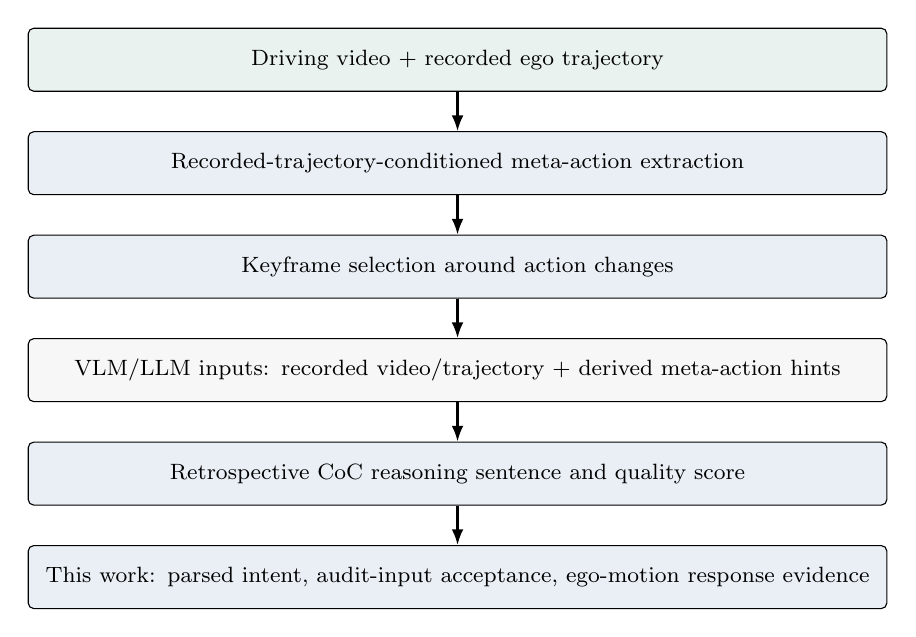
\begin{tikzpicture}[
  node distance=5mm,
  box/.style={draw, rounded corners=2pt, align=center, minimum height=8mm,
    text width=0.88\columnwidth, font=\footnotesize},
  obs/.style={box, fill=observed!10},
  der/.style={box, fill=derived!10},
  ass/.style={box, fill=assumed!10},
  input/.style={box, fill=black!3},
  flow/.style={-{Latex[length=2mm]}, thick}
]
\node[obs] (a) {Driving video + recorded ego trajectory};
\node[der, below=of a] (b) {Recorded-trajectory-conditioned meta-action extraction};
\node[der, below=of b] (c) {Keyframe selection around action changes};
\node[input, below=of c] (d) {VLM/LLM inputs: recorded video/trajectory + derived meta-action hints};
\node[der, below=of d] (e) {Retrospective CoC reasoning sentence and quality score};
\node[der, below=of e] (f) {This work: parsed intent, audit-input acceptance, ego-motion response evidence};
\draw[flow] (a) -- (b);
\draw[flow] (b) -- (c);
\draw[flow] (c) -- (d);
\draw[flow] (d) -- (e);
\draw[flow] (e) -- (f);
\end{tikzpicture}

\caption{CoC 추론 주석 생성과 본 논문 검증 입력으로의 변환. 자동 레이블링은 기록된 궤적에서 메타 행동을 먼저 도출하므로, 생성 문장은 온라인 인과 증명이 아니라 회고적 추론 지도 신호로 해석된다.}
\label{fig:annotation-flow}
\end{figure}

학습 관점에서 추론 주석은 기존 E2E 궤적 샘플을 확장하는 보조 목표이다. 일반적인 E2E 샘플이 관측 이력 $x_t$와 미래 궤적 $y_t$의 쌍이라면, 추론 보강형 샘플은 인과 문장 $z_t$를 추가해 $(x_t,z_t,y_t)$ 또는 쌍 목표 $(z_t,y_t)$를 구성한다. Alpamayo는 이런 방향의 대표 사례로 CoC 문장과 궤적 예측을 연결해 긴 꼬리 주행 일반화를 목표로 한다 \cite{wang2025alpamayo}. 그러나 본 논문은 실제 E2E 모델을 미세조정하지 않고, 생성된 추론 주석과 기록 자차 움직임이 검증 가능한 에피소드 궤적을 이루는지 다룬다.

그림~\ref{fig:annotation-flow}에서 중요한 지점은 메타 행동 추출이 기록된 궤적에 조건화되어 CoC 생성보다 먼저 수행된다는 것이다. 즉 CoC 문장은 주행 중 온라인으로 산출된 제어 판단이 아니라, 기록된 영상과 궤적을 함께 본 뒤 생성된 회고적 설명이다. 따라서 CoC와 같은 궤적 사이의 일치는 독립적인 인과 증거가 아니다. 이 때문에 본 논문은 CoC 문장을 직접 제어 명령으로 해석하지 않고, 검증기가 확인할 파싱된 추상 행동 의도와 연구자 선택 후보 시간 계약의 입력으로만 사용한다.

\subsection{감사 입력 선별 흐름}
청크~0에서의 감사 입력은 다음의 축소 흐름으로 구성된다.
\begin{quote}
\small
403 CoC 주석 $\rightarrow$ 290 기계 품질 통과 주석 $=134$ 방향 명시 주석 사건별 후보 계약 $+156$ 제외 $\rightarrow$ 130 속도 탐지기 사례 $+$ 4 이미 충족된 사례.
\end{quote}
290개 품질 통과 사건 중 156개는 영어 정규식 기반 의도 파서에서 방향이 모호하거나 비방향적이거나 복합 의도로 판정되어 제외했고, 추론 범위를 방향이 명시된 134개 사건으로 제한했다. 이 134건은 단일 이벤트 선별의 \emph{주석 사건별 후보 계약} 134개이다. 반복 사건끼리 같은 응답 시작을 공유할 수 있으므로 독립 응답 134개를 뜻하지 않으며, \preserve/\reset 상태 분석은 선택한 에피소드 사례에만 적용했다. 즉 $134=125+4+5$이며, 기본 분석 설정에서는 125개 속도 변화 계약 통과, 4개 이미 충족된 계약 통과, 5개 검토 후보로 분기한다. 이 수는 기록 전체 또는 403개 주석 전체에 대한 안전 판정이 아니다.

초기 기본 탐지기 선별에서는 검토 후보가 8건이었다. 이후 STOP/YIELD 사건 시점의 속도가 $0.5$~m/s 이하이면 이미 충족된 것으로 처리하는 규칙을 사후 추가하여 \texttt{scene-0046@10000000}, \texttt{scene-0159@4500000}, \texttt{scene-0159@4900000}을 재분류했고 후보가 5건이 되었다. 이 $0.5$~m/s 임계값은 요구사항에서 독립적으로 도출한 값이 아니라 해당 코호트에 맞춘 탐색적 보정 논리이다.

여기서 \texttt{quality\_pass}는 Qwen/Qwen3.5-35B-A3B가 생성한 \emph{기계 생성 감사 입력 수락 신호}이다. 상류 README에는 \texttt{Qwen/Qwen3.5-35B-A3B}라는 모델명은 기록되어 있으나, 불변 모델 스냅샷·태그·해시와 자동 레이블러 커밋은 보존되어 있지 않다. 따라서 특정 리비전을 추정하지 않으며, 이 누락을 재현성 한계로 취급한다. 이는 인간 정답(human gold)이나 주석 내용의 사실성을 보증하는 표지가 아니다. 다섯 검토 후보에 대한 시각 점검도 각 후보의 전방 카메라 네 프레임을 사용한 AI 시각 분류(triage)이며, 독립적인 인간 검증이 아니다. 이 점검은 검토 우선순위를 돕는 보조 문맥일 뿐 CoC--궤적 일치의 독립 인과 근거나 물리 안전성 결론을 제공하지 않는다.

\subsection{데이터 한 건의 실제 구조}
CoC-Nusc 추론 파일은 \texttt{data/baseline/coc\_nusc/reasoning/ood\_reasoning.parquet}이며, \texttt{clip\_id}별 행 안에 \texttt{events} JSON 문자열이 저장된다. 각 사건이 하나의 추론 보강형 레코드이다. 핵심 필드는 \texttt{clip\_id}, \texttt{event\_start\_timestamp}, \texttt{cot}, \texttt{quality}, \texttt{quality\_pass}이다.

\noindent\begin{minipage}{\columnwidth}
\begin{lstlisting}[caption={scene-0001의 CoC 사건 레코드 예시. 점수는 모델이 생성한 검증 신호이다.},label={lst:coc-record}]
{
  "clip_id": "scene-0001",
  "event_start_timestamp": 2500000,
  "cot": "Decelerate to maintain a safe distance from
          the lead truck ahead while navigating through
          the construction zone.",
  "quality": {
    "visual_evidence_score": 0.90,
    "behavior_match_score": 0.95,
    "decision_supported_by_video": 0.75,
    "causal_consistency_score": 0.70
  },
  "quality_pass": true
}
\end{lstlisting}
\end{minipage}

같은 \texttt{clip\_id} 안의 CoC 주석 사건 목록을 시간순으로 정렬하면 에피소드 궤적이 된다. \texttt{scene-0001}에는 2.5초, 3.5초, 4.8초에 트럭/공사 구간 관련 감속 추론이 반복되고, 6.3초에는 좌측 회피 추론이 나타나며, 9.3초에는 낮은 품질의 사건이 나타난다. 자차 움직임 보조 파일은 \texttt{data/baseline/coc\_nusc/labels/egomotion/scene-0001.egomotion.parquet}이며 타임스탬프, 위치, 쿼터니언, 속도, 가속도, 곡률 등을 포함한다. 본 논문은 $v=\sqrt{v_x^2+v_y^2}$로 자차 속도를 계산하고, CoC 주석 사건 이후의 지속적 속도 변화를 자차 움직임 응답 증거로 도출한다.

\subsection{증거 수준 구분}
모든 사건과 전환은 네 수준으로 구분한다. 이 구분은 ``검증 도구가 실행되었다''는 사실이 ``차량이 안전하다''는 주장으로 확대 해석되는 것을 방지하기 위해 필요하다.

\begin{table}[t]
\centering
\caption{증거 수준과 허용되는 주장.}
\label{tab:evidence-level}
\footnotesize
\begin{tabularx}{\columnwidth}{L{0.24\columnwidth}YY}
\toprule
Level & Example & Allowed claim \\
\midrule
Observed evidence & \texttt{cot}, timestamp, camera frame, ego-motion row & The record exists in the data \\
Derived evidence & Intent, ego speed, response onset, latency & The response is computed under stated rules \\
Synthetic assumption & $D$, repeat semantics, detector setting & Candidate requirements and sensitivity are tested \\
Synthetic mutation & No response, clock reset, overwrite, orphan response & Queries detect injected known faults \\
\bottomrule
\end{tabularx}
\end{table}

표~\ref{tab:evidence-level}에서는 표~\ref{tab:provenance-stack}의 출처 계층을 주장 수준으로 다시 번역한다. 관측 증거는 ``데이터에 그렇게 기록되어 있다''는 주장만 허용하고, 도출 증거는 ``정해진 규칙으로 계산했다''는 주장만 허용한다. 합성 가정과 합성 변이는 모델 체킹 절차를 시험하기 위한 입력이므로, 학습용 정상 궤적이나 실제 위험 사례로 바로 승격하지 않는다.

원천 근거가 있는 계약 통과(PASS)는 약한 유지 후보가 될 수 있지만, 합성 변이는 검사기 회귀 시험 전용이다. 기한이 독립 요구사항으로 정당화되지 않은 검토 후보(FAIL)는 학습용 위험 레이블이 아니다. 장면 간 연속성 증거가 없으면 출처 불충분으로 기록하고 장기 시퀀스 샘플로 묶지 않으며, 독립 클립/창 샘플로만 유지한다.

\section{문제 정의}
\label{sec:problem}

\subsection{감사 계약의 의미}
본 논문에서 감사 계약(audit contract)은 CoC 주석 사건으로부터 구성하는 추상적인 판단--반응 시간 검사 단위이다. 이 계약은 법적 의무나 물리 안전 의무가 아니라, 자연어 주석의 의미를 감사 가능한 시간 검사로 변환하기 위해 연구자가 선택한 의미론이다. 각 계약은 다음의 세 증거 층을 명시적으로 연결한다: (1) 주석에서 파싱한 행동 의도, (2) 연구자가 선택한 후보 시간 계약, (3) 자차 움직임에서 도출한 응답 증거. 다음 튜플은 이 선택을 표현한다.

\begin{equation}
O_i = \langle \tau_i, a_i, h_i, D_i, R_{a_i}, q_i, s_i \rangle .
\end{equation}

여기서 $\tau_i$는 시작 시각, $a_i$는 \textsc{Decelerate}, \textsc{Stop}, \textsc{Yield}, \textsc{Accelerate} 같은 주석에서 파싱한 추상 행동 의도, $h_i$는 원인 표현, $D_i$는 \emph{후보 기한(candidate deadline)}, $R_{a_i}$는 자차 움직임 응답 증거에 적용할 연구자 선택 응답 술어, $q_i$는 감사 입력 수락 조건, $s_i$는 \textsc{Pending}, \textsc{Responded}, \textsc{Failed}와 같은 계약 상태이다. \texttt{quality\_pass}에 따른 감사 입력 수락 조건을 만족한 CoC 주석 사건은 \textsc{Pending} 상태의 후보 감사 계약을 열며, 다음 제한 시간 응답 제약으로 검사한다.

\begin{equation}
q_i=\mathrm{trusted}
\Rightarrow
\exists t_r \in [\tau_i,\tau_i + D_i) :
R_{a_i}(t_r).
\label{eq:obligation-contract}
\end{equation}

식~\eqref{eq:obligation-contract}에서 \(\mathrm{trusted}\)는 구현에 남겨 둔 코드 식별자로서, 인간 정답이나 참인 판단이 아니라 \texttt{quality\_pass}에 의한 감사 입력 수락을 뜻한다. 이 식은 수락된 CoC 주석 사건 이후 후보 기한 안에 파싱된 의도와 일치하는 자차 움직임 응답 증거가 관측되어야 함을 뜻한다. 예를 들어 수락된 CoC가 ``전방 트럭/공사 구간 때문에 감속한다''라고 기술하면 검사기는 이를 다음 후보 감사 계약으로 변환한다.

\begin{quote}
\small
\textsc{Decelerate} 의도가 파싱되었으므로, 기준 시점 이후 후보 기한 안에 자차 속도/궤적에서 감속 방향의 자차 움직임 응답 증거가 관측되어야 한다.
\end{quote}

이때 감사 계약은 자연어 CoC 문장이 곧바로 차량 제어 명령이라는 뜻이 아니다. 기대 응답은 액추에이터 명령이 아니라 자차 움직임에서 도출한 응답 증거이며, $R_{a_i}$의 구체적 계산은 다음 절의 응답 탐지기가 담당한다. 따라서 \texttt{E<> Obligation.Active} 질의는 수락된 CoC 주석 사건이 모델 안에서 무시되지 않고 검사 대상 후보 시간 계약으로 생성되었는지를 확인하는 도달 가능성 검사이다.

식~\eqref{eq:obligation-contract}의 계약 통과는 ``기록된 CoC 주석 사건과 자차 움직임 궤적이 선택된 감사 의미론 아래에서 일관적이다''는 뜻이다. 검토 후보는 이 선택된 의미론 아래 추가 확인이 필요하다는 뜻이다. 어느 쪽도 법적 의무 준수, 충돌 회피, 안전거리 만족, 액추에이터 수준 제어 가능성, 폐루프 정책 안전성을 의미하지 않는다. 이러한 물리 안전성 판단에는 상대 객체 거리, 상대 속도, 차량 동역학, 액추에이터 지연, 마찰 조건이 추가로 필요하다.

\subsection{단일 이벤트와 연속 에피소드}
단일 이벤트 검사는 각 CoC 주석 사건을 독립 샘플로 보고 사건마다 새 시계를 시작한다. 이 방식은 국소적인 행동--응답 매칭에는 유용하지만, 이전 사건에서 열린 대기 계약을 유지하지 못한다. 에피소드 수준 검사는 같은 물리 클립 안의 CoC 주석 사건들을 시간순으로 연결하고 대기 계약, 최초 시작 시각, 반복 사건 이력, 응답 매칭 상태를 유지한다.

두 방식의 차이는 반복 CoC 주석 사건에서 명확해진다. 첫 감속 CoC 주석 사건 후 같은 감속 주석이 반복되고 실제 응답이 한 번만 나타났을 때, 단일 이벤트 검사는 반복 사건 기준 빠른 응답으로 판정할 수 있다. 반면 에피소드 검사는 최초 계약 기준 지연 응답으로 판정할 수 있다. 반복의 의미론을 정의하지 않으면 어느 판정을 적용해야 하는지 결정할 수 없다.

\begin{table}[t]
\centering
\caption{단일 이벤트 검사와 에피소드 수준 검사 비교.}
\label{tab:event-vs-episode}
\footnotesize
\begin{tabularx}{\columnwidth}{L{0.27\columnwidth}YY}
\toprule
Item & Single-event check & Episode-level check \\
\midrule
Input & One label and a local future window & Ordered events/responses in the same clip \\
Clock & New clock per label & Preserve pending clock or explicitly reset \\
Repeated label & Independent sample & Repeat/replace/conflict/deduplicate \\
Response binding & Nearest local motion & Matched to accepted audit contract \\
Detectable faults & Delay/no response & Overwrite, orphan response, ordering, boundary \\
\bottomrule
\end{tabularx}
\end{table}

표~\ref{tab:event-vs-episode}는 본 논문이 단일 레이블 분류 문제가 아니라 에피소드 상태 관리 문제를 다룬다는 점을 요약한다. 단일 이벤트 검사는 구현이 간단하지만 반복 레이블이 기존 계약을 연장하는지, 교체하는지, 중복으로 병합하는지 알 수 없다. 에피소드 수준 검사는 이 상태를 명시적으로 보존하므로, 늦은 응답을 반복 사건 기준의 빠른 응답으로 잘못 학습하는 오류를 드러낼 수 있다.

\subsection{시간 계약과 응답 탐지기}
수락된 CoC 주석 사건이 발생하면 후보 감사 계약의 응답 검사가 시작된다. 방향성 응답은 반개구 후보 구간 $r_i-\tau_i<D_i$에서 시작되어야 한다. 현재 모델의 기한 실패 전환이 $r_i-\tau_i=D_i$에서 활성화되므로 등호 시점은 통과에 포함하지 않는다. 응답 시작 시각 $r_i$는 자차 속도 $v(t)$에서 구간 길이 $W$, 최소 속도 변화 $\delta$, 방향 일치 비율 $\rho$를 사용해 탐지한다. 방향 부호를 $\sigma_i\in\{-1,+1\}$라 하면 다음 조건을 만족하는 최초 시각을 자차 움직임 응답 증거의 시작 시각으로 둔다.

\begin{align}
\sigma_i[v(r_i+W)-v(r_i)] &\ge \delta,\\
\frac{1}{m}\sum_{k=1}^{m}\mathbf{1}\{\sigma_i\Delta v_k>0\} &\ge \rho.
\end{align}

기본 설정은 $W=0.5$초, $\delta=0.1$m/s, $\rho=0.7$이다. 민감도 분석에서는 $W\in\{0.25,0.5,1.0\}$초, $\delta\in\{0.05,0.1,0.2\}$m/s, $\rho\in\{0.5,0.7,0.9\}$의 27개 설정을 사용한다. \textsc{Stop} 또는 \textsc{Yield} 사건 시점의 속도가 $0.5$~m/s 이하이면 새 감속 없이 이미 충족된 것으로 처리한다. 이는 초기 후보 8건을 검토한 뒤 세 사건을 재분류하기 위해 도입한 코호트 보정 탐색 규칙이며 규범 임계값이 아니다.

\subsection{반복 사건의 의미론}
반복 CoC 주석 사건은 세 가지 대안 주석 정책으로 비교한다. \preserve는 최초 대기 계약의 기한을 유지하여 지연을 최초 사건 기준으로 해석한다. \reset은 반복 사건이 후보 기한 시계를 다시 시작한다고 본다. \dedup은 짧은 시간 안의 동등한 CoC 주석 사건을 하나로 병합한다. \preserve는 지연 해석을 바꾸는 한 정책이지 유일하게 올바른 정책이 아니다. \preserve/\reset/\dedup 중 무엇을 적용할지는 데이터가 자동으로 결정하지 않으며, 감사 전에 명시적으로 선택해야 하는 시스템 요구사항 또는 주석 정책이다.

에피소드 수준 계약은 기한 외에도 형식 정합성 속성을 가져야 한다. 응답 수는 수락된 계약 수를 초과할 수 없고, 활성 계약이 없을 때 발생한 응답은 고아 응답이다. 낮은 품질의 추론은 기존 수락 계약을 덮어쓸 수 없고, 연속성 증거가 없는 장면 경계에서는 대기 계약을 다음 장면으로 이월하지 않는다. 이 속성들은 차량 동역학 속성이 아니라 CoC 주석--자차 움직임 응답 증거 변환 절차가 지켜야 할 프로토콜 속성이다.

\section{제안 방법}
\label{sec:method}

\subsection{전체 절차}
본 논문은 CoC 추론 주석을 안전/위험 레이블이나 제어 명령으로 직접 사용하지 않는다. 방법은 문제 정의의 세 증거 층---주석에서 파싱한 행동 의도, 연구자가 선택한 후보 시간 계약, 자차 움직임에서 도출한 응답 증거---을 다음 네 구성요소로 연결한다. 각 구성요소는 어떤 입력이 관측값인지, 어떤 규칙이 연구자 선택인지, 어떤 출력이 검토 대상인지 분리한다.

\begin{enumerate}
\item \textbf{증거 수집기(evidence collector)}는 \texttt{clip\_id} 안에서 타임스탬프와 CoC 텍스트를 수집하고, \texttt{quality\_pass} 및 자차 움직임을 함께 보존한다. 이 구성요소는 텍스트의 정답성이나 물리 위험을 판정하지 않고, 관측된 입력과 그 출처만 고정한다.
\item \textbf{계약 컴파일러(contract compiler)}는 수집된 텍스트에서 행동 의도와 원인 표현을 파싱하고, 후보 기한 $D_i$, 반복 정책(\preserve/\reset/\dedup), 그리고 의도별 응답 술어 $R_{a_i}$를 명시한다. 즉, 수락된 사건을 문제 정의의 $O_i=\langle\tau_i,a_i,h_i,D_i,R_{a_i},q_i,s_i\rangle$라는 후보 감사 계약으로 컴파일한다. $D_i$, 반복 정책, $R_{a_i}$는 데이터가 자동으로 발견한 안전 한계가 아니라 감사 전에 선택한 의미론이다.
\item \textbf{상태 관찰자(state observer)}는 시간순 계약과 응답 사건을 소비하여 의무의 생성--대기--응답--실패 생명주기, 응답 매칭, 저품질 사건의 감사 수용 상태 덮어쓰기 금지, 그리고 장면 경계에서의 대기 의무 종료를 검사한다. 이 상태는 단일 레이블의 분류 결과가 아니라 에피소드 수준의 프로토콜 상태이다.
\item \textbf{결과 라우터(result router)}는 검사 출력을 계약 통과, 의미론/임계값 의존 검토, 출처 부족, 합성 변이 결과로 구분한다. 계약 통과는 선택된 계약 아래 기록과 도출 응답이 일관적이라는 뜻이며, 검토 또는 출처 부족은 안전/위험 차량 레이블로 승격하지 않는다. 합성 변이 결과는 별도의 내부 타당성 확인 경로로만 보낸다.
\end{enumerate}

따라서 이 절차의 출력은 차량 제어가 아니라, CoC 주석 사건과 자차 움직임 증거가 지정된 후보 시간 계약을 만족하는지에 대한 정형 판정과 검토 경로이다.

\begin{figure*}[t]
\centering
\resizebox{0.84\textwidth}{!}{%
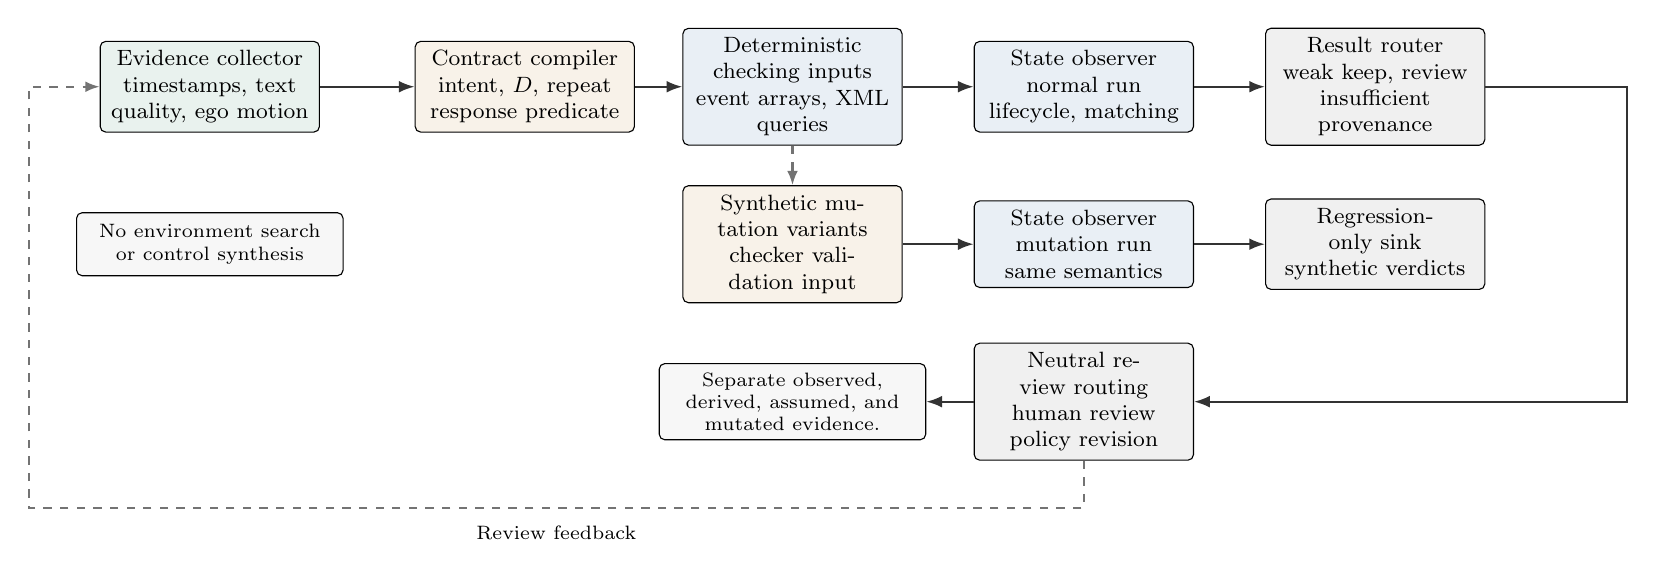
\begin{tikzpicture}[
  box/.style={draw, rounded corners=2pt, align=center, minimum height=11mm,
    text width=2.55cm, font=\footnotesize},
  small/.style={draw, rounded corners=2pt, align=center, minimum height=8mm,
    text width=3.15cm, font=\scriptsize},
  obs/.style={box, fill=observed!10},
  der/.style={box, fill=derived!10},
  ass/.style={box, fill=assumed!10},
  regression/.style={box, fill=neutral!8},
  route/.style={box, fill=neutral!8},
  note/.style={small, fill=black!3},
  flow/.style={-{Latex[length=2mm]}, thick, draw=black!80},
  feedback/.style={-{Latex[length=1.8mm]}, dashed, thick, draw=black!55}
]

% Four-component evidence architecture.
\node[obs] (collector) at (0,0) {Evidence collector\\timestamps, text\\quality, ego motion};
\node[ass] (compiler) at (4.0,0) {Contract compiler\\intent, $D$, repeat\\response predicate};
\node[der] (events) at (7.4,0) {Deterministic checking inputs\\event arrays, XML\\queries};
\node[der] (observer) at (11.1,0) {State observer\\normal run\\lifecycle, matching};
\node[route] (router) at (14.8,0) {Result router\\weak keep, review\\insufficient provenance};

\node[ass] (mut) at (7.4,-2.0) {Synthetic mutation variants\\checker validation input};
\node[der] (mutobserver) at (11.1,-2.0) {State observer\\mutation run\\same semantics};
\node[regression] (regression) at (14.8,-2.0) {Regression-only sink\\synthetic verdicts};
\node[note] (boundary) at (0,-2.0) {No environment search\\or control synthesis};

\node[route] (select) at (11.1,-4.0) {Neutral review routing\\human review\\policy revision};
\node[note] (scope) at (7.4,-4.0)
  {Separate observed, derived, assumed, and mutated evidence.};

\draw[flow] (collector) -- (compiler);
\draw[flow] (compiler) -- (events);
\draw[flow] (events) -- (observer);
\draw[flow] (observer) -- (router);
\draw[feedback] (events) -- (mut);
\draw[flow] (mut) -- (mutobserver);
\draw[flow] (mutobserver) -- (regression);
\draw[flow] (router.east) -- ++(1.8,0) |- (select.east);
\draw[flow] (select) -- (scope);

% Feedback is routed outside the node area to avoid crossing boxes.
\coordinate (feedbackleft) at ([xshift=-6mm]boundary.west);
\draw[feedback] (select.south) -- ++(0,-0.6) coordinate (feedbackbottom)
  -- node[midway,below=1mm,font=\scriptsize,align=center]{Review feedback}
  (feedbackbottom -| feedbackleft) -- (feedbackleft) |- (collector.west);

\end{tikzpicture}%
}

\caption{증거 수집기, 계약 컴파일러, 상태 관찰자, 결과 라우터로 구성한 제안 방법. 사람 검토는 중립적 후속 경로이고, 합성 변이는 동일한 관찰자 의미론의 별도 실행 인스턴스를 거쳐 회귀 시험 전용 출구로 분리한다.}
\label{fig:method-pipeline}
\end{figure*}

그림~\ref{fig:method-pipeline}에서 증거 수집기는 관측값을 보존하고, 계약 컴파일러는 그 값을 후보 시간 계약으로 변환하며, 상태 관찰자는 계약 상태를 검사하고, 결과 라우터는 판정의 사용 범위를 분리한다. 최종 검토 피드백은 원본 데이터를 바꾸지 않고 기한, 반복 의미론, 탐지기 임계값을 재검토하는 데만 사용한다.

\subsection{UPPAAL 네트워크}
\uppaal 모델은 단일 오토마타가 아니라 실험 목적마다 다른 템플릿 네트워크이다. \texttt{scene-0001} 모델에서는 증거 수집기가 고정한 타임스탬프, 텍스트, 품질, 자차 움직임과 계약 컴파일러가 만든 사건 배열을 사용한다. \texttt{CoCSource}는 감사 수용 시작, 반복, 감사 비수용 사건을 타임스탬프 순서로, \texttt{EgoTrace}는 자차 움직임에서 도출된 응답 증거를 그 순서대로 재생한다. 이 원천 오토마타는 \emph{결정적 기록 사건열}을 한 번 재생할 뿐, 차량 환경을 탐색하지 않으며 안전 제어를 생성하거나 제어 정책을 합성하지 않는다. \texttt{ObligationManager}, \texttt{ReactionObserver}, \texttt{DecisionValidator}는 같은 사건열에서 의무 생명주기, 응답 매칭, 반복 시계 정책과 저품질 덮어쓰기를 검사한다. 코호트와 체인 실험은 뒤의 표와 같이 별도 모델군이며, 하나의 통합 모델이 모든 실험에 실행된 것은 아니다.

\begin{figure*}[t]
\centering
\resizebox{0.78\textwidth}{!}{%
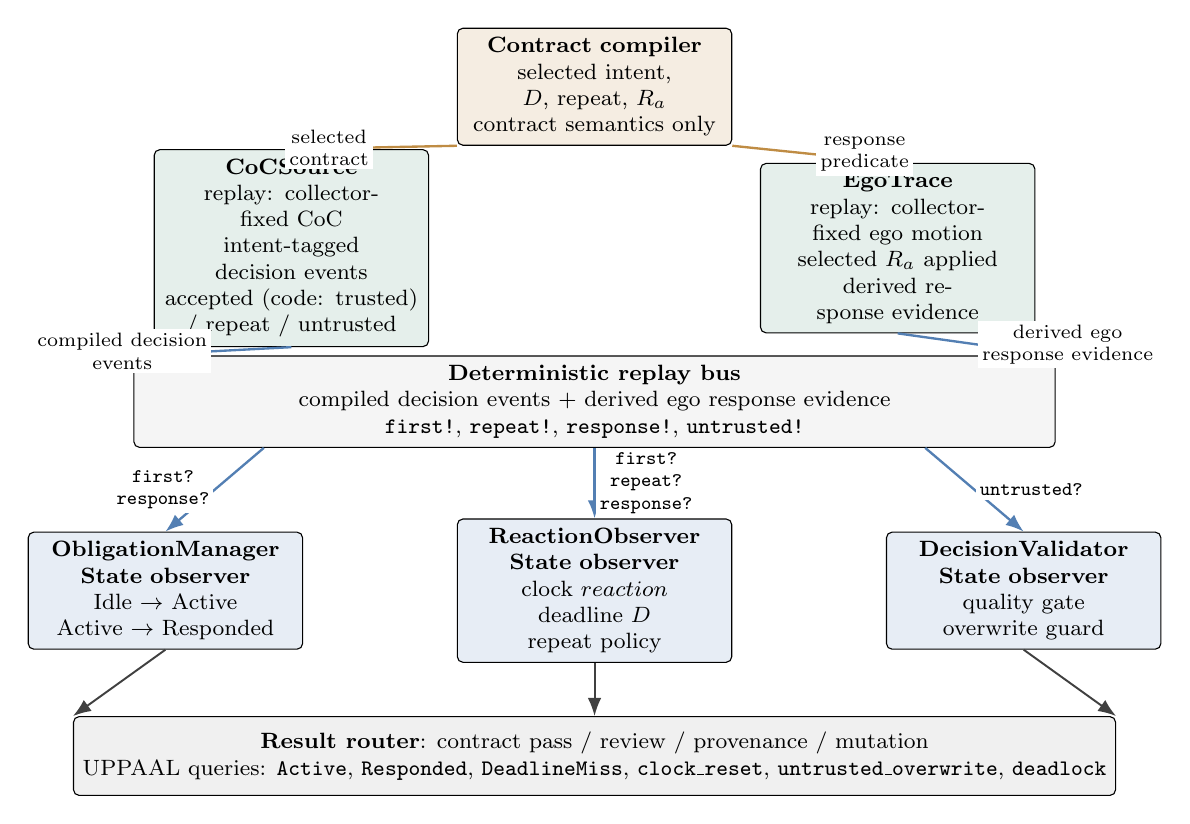
\begin{tikzpicture}[
  node distance=13mm and 15mm,
  box/.style={draw, rounded corners=2pt, align=center, minimum height=13mm,
    text width=3.25cm, font=\footnotesize},
  source/.style={box, fill=observed!12},
  monitor/.style={box, fill=derived!11},
  compiler/.style={box, fill=assumed!13},
  bus/.style={draw, rounded corners=2pt, fill=black!4, align=center,
    minimum width=11.7cm, minimum height=11mm, font=\footnotesize},
  flow/.style={-{Latex[length=2.3mm]}, line width=0.7pt, draw=black!75},
  event/.style={-{Latex[length=2.3mm]}, line width=0.85pt, draw=derived!80},
  audit/.style={-{Latex[length=2.3mm]}, line width=0.85pt, draw=assumed!85},
  label/.style={font=\scriptsize, align=center, fill=white, inner sep=1.5pt}
]

% Sources.
\node[source] (coc) at (0,3.4) {
  \textbf{CoCSource}\\
  replay: collector-fixed CoC\\
  intent-tagged decision events\\
  accepted (code: trusted) / repeat / untrusted
};

\node[source] (ego) at (7.7,3.4) {
  \textbf{EgoTrace}\\
  replay: collector-fixed ego motion\\
  selected $R_a$ applied\\
  derived response evidence
};

% Researcher-selected contract semantics, kept distinct from recorded evidence.
\node[compiler] (compiler) at (3.85,5.45) {
  \textbf{Contract compiler}\\
  selected intent, $D$, repeat, $R_a$\\
  contract semantics only
};

% Broadcast bus.
\node[bus] (bus) at (3.85,1.45) {
  \textbf{Deterministic replay bus}\\
  compiled decision events + derived ego response evidence\\
  \texttt{first!}, \texttt{repeat!}, \texttt{response!}, \texttt{untrusted!}
};

% Monitors.
\node[monitor] (obl) at (-1.6,-0.95) {
  \textbf{ObligationManager}\\
  \textbf{State observer}\\
  Idle $\rightarrow$ Active\\
  Active $\rightarrow$ Responded
};

\node[monitor] (react) at (3.85,-0.95) {
  \textbf{ReactionObserver}\\
  \textbf{State observer}\\
  clock $reaction$\\
  deadline $D$\\
  repeat policy
};

\node[monitor] (valid) at (9.3,-0.95) {
  \textbf{DecisionValidator}\\
  \textbf{State observer}\\
  quality gate\\
  overwrite guard
};

% Compiler selects contract semantics; sources replay the resulting evidence.
\draw[audit] (compiler.south west) -- node[label, left] {selected\\contract} (coc.north);
\draw[audit] (compiler.south east) -- node[label, right] {response\\predicate} (ego.north);

% Source to bus.
\draw[event] (coc.south) -- node[label, left] {compiled decision\\events} (bus.north west);
\draw[event] (ego.south) -- node[label, right] {derived ego\\response evidence} (bus.north east);

% Bus to monitors. Route from distinct bottom anchors to avoid visual crossing.
\draw[event] ([xshift=-4.2cm]bus.south) -- node[label, left] {\texttt{first?}\\\texttt{response?}} (obl.north);
\draw[event] (bus.south) -- node[label, right] {\texttt{first?}\\\texttt{repeat?}\\\texttt{response?}} (react.north);
\draw[event] ([xshift=4.2cm]bus.south) -- node[label, right] {\texttt{untrusted?}} (valid.north);

% Result box.
\node[draw, rounded corners=2pt, fill=neutral!8, align=center,
  minimum width=11.7cm, minimum height=10mm, font=\footnotesize] (queries)
  at (3.85,-3.05) {
  \textbf{Result router}: contract pass / review / provenance / mutation\\
  UPPAAL queries:
  \texttt{Active}, \texttt{Responded}, \texttt{DeadlineMiss},
  \texttt{clock\_reset}, \texttt{untrusted\_overwrite}, \texttt{deadlock}
};

\draw[flow] (obl.south) -- (queries.north west);
\draw[flow] (react.south) -- (queries.north);
\draw[flow] (valid.south) -- (queries.north east);

\end{tikzpicture}%
}

\caption{\texttt{scene-0001-normal}에 대응하는 \uppaal 네트워크 개념도. 증거 수집기와 계약 컴파일러의 결정적 사건열을 상태 관찰자가 소비하고, 결과 라우터가 질의 판정을 분리한다.}
\label{fig:uppaal-network}
\end{figure*}

그림~\ref{fig:uppaal-network}에서 위쪽 두 템플릿은 증거 수집기와 계약 컴파일러가 준비한 입력 흐름을 재생하는 원천이고, 아래쪽 세 템플릿은 상태 관찰자를 구성한다. 이 구분이 중요하다. \texttt{CoCSource}와 \texttt{EgoTrace}는 새로운 주행 행동을 탐색하지 않으며, 관찰자들은 이미 주어진 사건열 위에서 의무 생성, 응답 매칭, 기한 실패, 출처 덮어쓰기와 경계 정책을 검사한다. 질의 결과의 의미는 결과 라우터가 계약 통과, 의미론/임계값 의존 검토, 출처 부족, 합성 변이로 분리한다.

그림~\ref{fig:uppaal-network}의 블록도는 표~\ref{tab:ta-skeleton}의 시간 오토마타 네트워크로 구현된다. 시간 단위는 XML 내부에서 밀리초 정수이며, 표에서는 \texttt{first}, \texttt{repeat}, \texttt{response}, \texttt{untrusted}를 각각 \texttt{first\_trigger}, \texttt{repeat\_trigger}, \texttt{response}, \texttt{untrusted\_event} 방송 채널의 약어로 사용한다. 원천 템플릿은 사건을 한 번 재생하고, 관찰자 템플릿들은 같은 방송 사건에 동기화되어 의무의 생성, 기한, 반복 의미론, 낮은 품질 사건의 덮어쓰기 금지를 독립적으로 검사한다.

\begin{table}[!htbp]
\centering
\caption{그림~\ref{fig:uppaal-network}에 대응하는 시간 오토마타 골격.}
\label{tab:ta-skeleton}
\scriptsize
\setlength{\tabcolsep}{2.5pt}
\renewcommand{\arraystretch}{0.90}
\begin{tabularx}{\columnwidth}{L{0.26\columnwidth}L{0.21\columnwidth}Y}
\toprule
Template & Locations and clocks & Main transitions and meaning \\
\midrule
\texttt{CoCSource} &
\texttt{C0--C4}, \texttt{episode} &
$0$s \texttt{first!}; $1.0$s, $2.3$s \texttt{repeat!}; $6.8$s \texttt{untrusted!}. Replays CoC decision events in timestamp order. \\
\midrule
\texttt{EgoTrace} &
\texttt{E0--E1}, \texttt{episode} &
$2.16$s \texttt{response!}. Replays weak response evidence derived from ego speed. \\
\midrule
\texttt{ObligationManager} &
\texttt{Idle}, \texttt{Active}, \texttt{Responded} &
Opens an obligation on \texttt{first?}; closes it on \texttt{response?}. Deadline state is tracked separately. \\
\midrule
\texttt{ReactionObserver} &
\texttt{Idle}, \texttt{Armed}, \texttt{Done}, \texttt{DeadlineMiss}; clock \texttt{reaction} &
Sets \texttt{reaction=0} on \texttt{first?}; the contract requires response before \texttt{reaction}$=D$, where the miss transition becomes enabled. \preserve does not restart \texttt{reaction} on repeats. \\
\midrule
\texttt{DecisionValidator} &
\texttt{Clean}; Boolean overwrite flag &
Keeps one location and sets the Boolean on \texttt{untrusted?} when the mutation enables an overwrite. \\
\bottomrule
\end{tabularx}
\end{table}

표~\ref{tab:ta-skeleton}에서는 그림~\ref{fig:uppaal-network}의 각 블록이 실제 모델에서 어떤 위치와 전환으로 구현되는지 정리한다. 예를 들어 \texttt{CoCSource}의 \texttt{first!} 전환은 의무 생성을 촉발하고, \texttt{EgoTrace}의 \texttt{response!} 전환은 자차 속도에서 도출한 응답 증거를 방송한다. \texttt{ReactionObserver}는 이 두 사건 사이의 지역 시계 \texttt{reaction}을 검사하며, \preserve 기준 모델에서는 반복 사건을 보더라도 \texttt{reaction}을 재시작하지 않는다. 저장 집계에는 구현 시계가 기한과 같은 \texttt{reaction}$=D$인 사례가 없으며, 등호 시점의 전환 우선순위를 직접 고정하는 검사기 회귀 시험은 후속 과제로 남긴다.

\begin{table}[!htbp]
\centering
\caption{실험별 \uppaal 모델군.}
\label{tab:model-families}
\scriptsize
\begin{tabularx}{\columnwidth}{L{0.25\columnwidth}L{0.30\columnwidth}Y}
\toprule
Experiment & Templates & Purpose \\
\midrule
\texttt{scene-0001} & \texttt{CoCSource}, \texttt{EgoTrace}, \texttt{ObligationManager}, \texttt{ReactionObserver}, \texttt{DecisionValidator} & Five-template timed lifecycle and mutation check \\
\midrule
94-scene cohort & \texttt{EpisodeSource}, \texttt{LineageMonitor} & Two-template flag/query serialization regression \\
\midrule
13-chain smoke artifact & \texttt{LoopSource}, \texttt{Monitor} & Two-template implementation pipeline smoke test with a distinct parser/detector \\
\bottomrule
\end{tabularx}
\end{table}

이 골격에서 \texttt{CoCSource}와 \texttt{EgoTrace}는 환경을 새로 생성하는 반응형 제어기가 아니라, 관측 및 도출 증거 흐름을 결정적으로 재생하는 원천 오토마타이다. 반대로 \texttt{ObligationManager}, \texttt{ReactionObserver}, \texttt{DecisionValidator}는 같은 사건 흐름을 서로 다른 관점에서 감시하는 상태 관찰자 오토마타이다. 따라서 시간 오토마타의 검증 대상은 ``차량이 안전하게 주행했는가''가 아니라 ``감사 입력으로 수용된 CoC 주석 사건이 후보 의무를 열었는가'', ``반복 사건이 시계를 부당하게 초기화하지 않았는가'', ``응답 증거가 후보 기한 안에 매칭되었는가'', ``저품질 사건이 수용된 상태를 덮어쓰지 않았는가'', ``연속성 증거가 없는 경계에서 대기 의무가 닫혔는가''이다.

단일 결정적 재생만 실행한다면 동일한 기한 검사는 일반 스크립트로도 계산할 수 있다. 본 논문에서 모델 체킹을 사용하는 이유는 각 모델군의 상태 관찰자, 반복 의미론, 경계 정책 또는 변이 오라클을 선언하고, 위반 시 어떤 관찰자가 어떤 시각에 실패했는지 반례 궤적으로 얻기 위해서이다. 특히 \texttt{scene-0001} 모델은 같은 원천 사건을 의무 생명주기, 기한 관찰자와 출처 검증기가 동시에 소비하도록 만들기 때문에, 단순 수치 계산보다 ``어떤 정책 조합에서 어떤 프로토콜 속성이 깨졌는가''를 명세 수준에서 검토할 수 있다.

\subsection{scene-0001의 의미론 변환}
\texttt{scene-0001}의 원본 및 도출 정보는 표~\ref{tab:scene1-map}처럼 \uppaal 사건으로 변환된다. 표에서는 가독성을 위해 원본 타임스탬프를 장면 내부 초 단위로 표시하고, \uppaal 사건 시각은 최초 감사 수용 시작 사건을 기준으로 한 상대 초 단위로 표시한다. 실제 XML 생성 시에는 이 값을 밀리초 정수로 양자화한다.

\begin{table}[!htbp]
\centering
\caption{\texttt{scene-0001} 증거를 \uppaal 사건으로 변환한 예. 시간 단위는 초이다.}
\label{tab:scene1-map}
\footnotesize
\begin{tabularx}{\columnwidth}{L{0.30\columnwidth}L{0.25\columnwidth}Y}
\toprule
Source/derived evidence & \uppaal event & Meaning \\
\midrule
$t=2.500$s, audit-accepted \textsc{Decelerate} & \texttt{first!} at $0.000$s & Opens the first deceleration obligation \\
$t=3.500$s, repeated \textsc{Decelerate} & \texttt{repeat!} at $1.000$s & Observes a repeat of the same obligation \\
$t=4.660$s, speed-decrease onset & \texttt{response!} at $2.160$s & Weak response derived from ego trajectory \\
$t=4.800$s, repeated \textsc{Decelerate} & \texttt{repeat!} at $2.300$s & Repeated label after response evidence \\
$t=9.300$s, low-quality CoC & \texttt{untrusted!} at $6.800$s & Code-named event that must not overwrite audit-accepted state \\
\bottomrule
\end{tabularx}
\end{table}

표~\ref{tab:scene1-map}의 \texttt{first!}, \texttt{repeat!}, \texttt{untrusted!}는 각각 생성 XML의 \texttt{first\_trigger!}, \texttt{repeat\_trigger!}, \texttt{untrusted\_event!} 채널을 줄여 표기한 것이다.

생성되는 대표 질의는 다음과 같다.

\noindent\begin{minipage}{\columnwidth}
\begin{lstlisting}[caption={대표 \uppaal 질의 집합.},label={lst:queries}]
E<> Obligation.Active
E<> Obligation.Responded
A[] not Reaction.DeadlineMiss
A[] not clock_reset_violation
A[] not untrusted_overwrite
A[] not orphan_response
A[] not boundary_violation
A[] not deadlock
\end{lstlisting}
\end{minipage}

본 연구의 \uppaal 모델은 폐루프 반응형 제어기가 아니다. 기록된 CoC 사건 흐름과 자차 움직임 응답 흐름을 재생하고 관찰자 오토마타가 프로토콜 수준 속성을 검사한다. 따라서 \uppaal은 환경을 탐색하거나 안전 제어를 생성하지 않는다. 단일 결정적 재생 하나의 PASS만으로는 모델 체킹 의미가 크지 않다. 본 논문에서 \uppaal의 가치는 여러 관찰자, 반복 의미론, 변이 오라클, 다중 장면 경계 정책을 같은 정형 프레임워크 안에서 선언적으로 결합하고 반례 궤적을 얻는 데 있다.

\subsection{합성 변이 오라클}
합성 변이 오라클은 결과 라우터가 정상 계약 통과와 알려진 프로토콜 결함을 구분하는지 확인하는 \emph{검사기 내부 타당성} 장치이다. 기준 모델의 PASS가 질의 비활성화나 모델 구성 오류로 생긴 결과가 아님을 점검하기 위해, 정상 궤적과 함께 의도적으로 결함을 삽입한 변이 모델을 만들고 각 변이의 기대 실패 질의와 비교한다. 이 검사는 실제 오류 검출률, 실제 주행 결함의 발생 빈도 또는 미관측 배치 행동을 추정하지 않는다.

\begin{table}[!htbp]
\centering
\caption{변이 오라클과 기대 실패 속성.}
\label{tab:mutation-oracle}
\footnotesize
\begin{tabularx}{\columnwidth}{L{0.28\columnwidth}YY}
\toprule
Mutation & Injected fault & Expected failure \\
\midrule
\texttt{deadline\_2s} & Shrink deadline while keeping response & Deadline query \\
\texttt{no\_response} & Remove ego response & Response reachability, deadline \\
\texttt{clock\_reset} & Restart clock on repeat & Clock-reset query \\
\texttt{untrusted\_ovr.} & Low-quality event overwrites audit-accepted state & Provenance query \\
\texttt{orphan\_response} & Remove obligation trigger but keep response & Orphan-response query \\
\texttt{late\_stop} & Delay stop/hold stage & Stage deadline \\
\texttt{premature\_rec.} & Recover before hazard clearance & Clearance precondition \\
\bottomrule
\end{tabularx}
\end{table}

표~\ref{tab:mutation-oracle}의 \texttt{untrusted\_ovr.}와 \texttt{premature\_rec.}는 각각 \texttt{untrusted\_overwrite}와 \texttt{premature\_recovery} 변이를 축약한 것이다. 변이는 실제 데이터 결함이라고 주장하기 위한 것이 아니다. 검사기와 질의 집합이 알려진 프로토콜 결함을 구분할 수 있는지 확인하기 위한 합성 시험이며, 정상 궤적 지도 신호나 실제 오류 검출률의 근거로 사용해서는 안 된다.

\subsection{다중 장면 확장}
로컬 CoC-Nusc 단독 데이터에는 장면 간 전역 타임스탬프, 로그 식별자, 이전/다음 관계, 전역 자차 자세가 부족하다. 따라서 기본 정책은 모든 장면을 독립 에피소드로 닫고 장면 경계를 넘어 대기 의무를 이월하지 않는 것이다. 이 정책은 오류 차단 시험으로 사용된다. 연속성 증거가 없는 경계에서 의무가 다음 장면까지 살아 있으면 변환 절차의 오류로 판정한다.

연속성이 입증된 경우에는 여러 장면을 하나의 장기 에피소드로 연결할 수 있다. 예비 실험에서는 nuScenes 호환 메타데이터 미러를 사용해 같은 로그의 인접 장면 쌍을 찾고, 간격이 1초 이하이며 로컬 추론/자차 움직임이 있는 장면들을 체인으로 묶었다. 이후 각 장면 내부 사건 타임스탬프에 전역 장면 오프셋을 더해 하나의 시간선을 만들고, 루프 인덱스 방식의 \uppaal 모델로 검증했다. 루프 인덱스 모델은 사건마다 전환을 모두 쓰는 대신 \texttt{idx}, \texttt{event\_time[]}, \texttt{event\_kind[]}, \texttt{event\_gap[]} 배열을 사용하므로, 장면 수가 늘어나도 오토마타 구조는 유지되고 데이터 배열만 커진다.

\section{실험 설계}
\label{sec:experiments}

본 절은 여덟 개의 독립 실험 나열 대신, 증거 수집기--계약 컴파일러--상태 관찰자--결과 라우터의 네 구성요소가 어떤 입력을 고정하고 어떤 정책을 비교하는지를 세 증거 블록으로 정리한다. 모든 블록에서 CoC 텍스트, 품질 상태, 자차 움직임, 메타데이터는 관측 또는 도출 입력으로 보존하고, 기한ㆍ반복 정책ㆍ응답 탐지 임계값은 연구자가 명시한 감사 의미론으로 다룬다. 따라서 출력의 PASS/FAIL은 선택한 후보 시간 계약의 통과 또는 검토 경로이며, 차량의 물리 안전/위험 레이블이나 폐루프 제어 성능을 뜻하지 않는다.

\subsection{실험 블록 A: 변환·검사기 타당성}
\label{sec:exp-block-a}

블록 A는 \texttt{scene-0001}과 그 결정적 사건열을 고정한 채, 증거 수집기가 보존한 CoC 시점ㆍ품질ㆍ자차 속도와 계약 컴파일러가 만든 \preserve, $D=3$초 계약을 상태 관찰자가 올바르게 소비하는지 확인한다. 기준 입력에는 최초 2.5초 \textsc{Decelerate} 사건, 3.5초와 4.8초의 반복 사건, 4.6597초에 도출한 자차 속도 응답 시작, 낮은 품질 사건이 포함된다. 정상 모델의 의무 생성ㆍ응답ㆍ기한ㆍ반복 시계ㆍ출처ㆍ교착 질의와 함께, 응답 또는 출처 계보를 의도적으로 훼손한 \texttt{deadline\_2s}, \texttt{clock\_reset}, \texttt{no\_response}, \texttt{untrusted\_overwrite} 합성 변이를 비교한다. 출력은 정상 및 변이별 질의 판정 벡터와 알려진 변이에 대한 기대 오라클 일치이며, 결과 라우터는 이를 검사기 내부 타당성 결과로만 분리한다.

같은 블록에서 \texttt{scene-0001-chained}의 \textsc{Follow} $\rightarrow$ \textsc{Decelerate} $\rightarrow$ \textsc{Stop/Hold} $\rightarrow$ \textsc{Recover} 프로토콜도 비교한다. 관측 CoC 감속 요청과 자차 움직임 응답은 고정하지만, \textsc{Stop/Hold/Recover} 시점은 합성 프로토콜 가정으로 명시하고 \texttt{late\_stop}, \texttt{skip\_hold}, \texttt{premature\_recovery}, \texttt{no\_recovery}의 단계ㆍ순서ㆍ복구 결함을 주입한다. 이 비교의 출력은 각 합성 결함에 대응하는 단계, 순서, 기한, 위험 해소 및 교착 질의의 판정이다.

블록 A의 증거는 RQ1의 \texttt{scene-0001} 변환ㆍ알려진 변이 구분과 RQ4의 정형 관찰자 부가가치에만 대응한다. 이는 실제 오류 검출률, 합성 다단계 궤적의 학습용 적합성 또는 차량 안전을 입증하지 않는다. 메타데이터 미러의 13개 체인과 스크립트 일치 집계는 이 블록의 공유 계약 검증에서 제외하고 블록 C의 구현별 기본 동작 기록으로 분리한다.

\subsection{실험 블록 B: 일괄 감사와 민감도}
\label{sec:exp-block-b}

블록 B는 청크 0의 기록된 94개 장면과 403개 CoC 주석, 해당 자차 움직임 궤적을 고정한다. 증거 수집기는 이 입력에서 290개 \texttt{quality\_pass} 주석을 보존한다. 영어 정규식/복합 의도 규칙에서 방향이 명시된 134개 주석 사건별 후보 계약을 포함하고, 모호하거나 비방향적이거나 복합 의도인 156개는 제외한다($290=134+156$). 134건 중 130개는 속도 변화 탐지기 대상이고, 나머지 4개는 사건 시점에 정지 또는 양보 조건을 이미 만족한 \texttt{PASS\_ALREADY\_SATISFIED} 사건이다. 반복 사건은 같은 응답 시작을 공유할 수 있고 상태형 \preserve/\reset 검사는 선택 에피소드에만 적용한다. 기준 $D=3$초와 \preserve 정책을 기준점으로 두고, \preserve/\reset/\dedup 반복 정책, $D=1,2,3,4,5$초 후보 기한, 그리고 창ㆍ속도 변화 임계값ㆍ방향 비율을 각각 3단계로 조합한 27개 탐지기 설정을 비교한다.

일괄 출력은 94개 장면의 감사 라우팅, 기본 설정의 다섯 검토 후보(\texttt{scene-0019}, \texttt{scene-0028}, \texttt{scene-0042}, \texttt{scene-0065}, \texttt{scene-0074}), 반복 의미론 및 후보 기한에 따른 판정 변화, 그리고 130개 탐지 대상에 대한 27설정 민감도이다. 최초 기본 탐지기 후보는 8건이었고, AI 선별 뒤 $v\leq0.5$~m/s인 STOP/YIELD를 이미 충족으로 처리하는 코호트 보정 탐색 규칙을 사후 추가해 \texttt{scene-0046@10000000}, \texttt{scene-0159@4500000}, \texttt{scene-0159@4900000}을 재분류하여 5건이 되었다. 동시에 94개 장면 레이블의 위반 불리언을 기준ㆍ출처 변이ㆍ응답 변이 모델에 직접 직렬화하여 282개 모델과 1,128개 질의의 기대 판정을 확인한다. 기대 판정도 같은 레이블에서 도출되므로 이는 관찰자 수준 시간 변이 검증이 아니라 플래그/질의 직렬화 회귀이다. 관찰자 수준 시간 변이 근거는 \texttt{scene-0001} 모델에 한정한다.

\begin{table}[t]
\centering
\caption{일괄 감사 블록의 기록된 입력과 생성 범위.}
\label{tab:batch-size}
\begin{tabular}{lr}
\toprule
Item & Value \\
\midrule
Scenes & 94 \\
CoC annotations & 403 \\
Quality-passing annotations & 290 \\
Applicable longitudinal contracts & 134 \\
Speed-change detector subset & 130 \\
Serialized cohort variants & 282 \\
Flag/query regression evaluations & 1,128 \\
\bottomrule
\end{tabular}
\end{table}

따라서 블록 B의 출력은 물리적 결과가 아니라 동일 기록에 대해 어떤 감사 정책과 응답 증거 설정이 검토 우선순위를 바꾸는지의 라우팅ㆍ민감도 결과이다. 403개 주석 전체의 안전성, 다섯 후보의 실제 결함, 단일 탐지기 설정의 보편적 타당성, 또는 $D=3$초의 차량 안전 임계값으로 외삽해서는 안 된다. 이 블록은 RQ2에만 대응한다.

\subsection{실험 블록 C: 출처와 에피소드 확장}
\label{sec:exp-block-c}

블록 C는 ``연결할 수 있는가''라는 출처 적격성 판단과 ``연결 후 시간 계약이 통과하는가''라는 사후 감사 판단을 분리한다. 먼저 로컬 CoC-Nusc의 장면별 시간ㆍ자세 초기화와 장면 간 로그/이전ㆍ다음 관계 부재를 고정하고, 모든 장면을 독립 에피소드로 닫는 정책을 오류 차단 시험으로 사용한다. 합성 두 장면 시간선에서는 장면 A의 감사 수용 요청 주석 사건(0ms), 검증되지 않은 경계(1000ms), 장면 B의 응답 증거(1500ms), 기한(3000ms)을 고정한다. 올바른 \texttt{correct\_discard}와 결함 \texttt{buggy\_carryover}를 비교하여, 상태 관찰자가 경계에서 대기 의무를 \texttt{Discarded}로 닫고 교차 경계 완료와 이월을 금지하는지 검사한다. 출력은 원천 완료, 폐기 도달성, 교차 완료 금지, 이월 금지, 교착 질의의 판정이다.

그 다음 공식 mini는 연속성 스키마를 확인하는 용도로만 사용하고, trainval 후보의 적격성은 로컬 심볼릭 링크로 보관한 nuScenes 호환 메타데이터 미러에서 별도로 감사한다. 같은 로그의 인접성, 1초 이하 간격, 양쪽 장면의 로컬 추론과 자차 움직임 존재를 연속성 적격 조건으로 고정해 16개 엄격 쌍과 13개 체인을 구성했다. 다만 보존된 체인 산출물은 공유 계약과 다른 구현을 사용한다. \texttt{generate\_multiscene\_chain\_model.py}는 느린 의도 토큰을 먼저 찾는 부분문자열 파서라서 ``yield ... then accelerate'' 같은 복합 의도를 감속으로 오분류할 수 있고, 응답 탐지기는 $W=1.0$초, $\delta=0.7$~m/s이며 방향 비율 $\rho$를 사용하지 않는다. 이 사건 배열을 \texttt{LoopSource}/\texttt{Monitor} 두 템플릿에 넣은 13체인 결과와 스크립트 비교는 구현 파이프라인이 끝까지 실행되었는지 보는 스모크 테스트로만 보존한다.

블록 C에서 RQ3의 직접 근거는 로컬 장면 독립성 및 경계 오류 차단 시험이다. 로컬 장면 독립성은 연속 주행의 부정 증거가 아니라 출처 부족 시 의무 이월을 차단하는 정책이다. 13체인 산출물의 수치는 공유 계약의 기한ㆍ응답 또는 장기 에피소드 일반화 근거가 아니며, 공식 trainval 시퀀스 인증이나 객체ㆍ위험 연속성 증명에도 사용할 수 없다.

\begin{table*}[t]
\centering
\caption{실험 블록, 연구 질문, 그리고 해석 경계.}
\label{tab:experiment-rq-map}
\begingroup
\scriptsize
\setlength{\tabcolsep}{2.5pt}
\renewcommand{\arraystretch}{0.90}
\begin{tabularx}{\textwidth}{@{}L{0.14\textwidth}L{0.19\textwidth}L{0.23\textwidth}L{0.18\textwidth}L{0.08\textwidth}Y@{}}
\toprule
실험 블록 & 고정 조건 & 조작·비교 조건 & 출력 & 대응 RQ & 해석 범위 \\
\midrule
블록 A: 변환·검사기 타당성 & \texttt{scene-0001}의 CoCㆍ품질ㆍ자차 응답 사건열 & 응답ㆍ출처 변이, 합성 다단계 결함 & 질의/시간 변이 오라클 판정, 관찰자ㆍ교착 명세 범위 & RQ1, RQ4 & 알려진 합성 결함의 구분과 명세 조합만 지지한다. 실제 오류 검출률, 합성 궤적의 학습 적합성, 차량 안전으로 외삽하지 않는다. \\
\midrule
블록 B: 일괄 감사와 민감도 & 94장면ㆍ403주석의 기록 궤적; 290 품질 통과, 134 방향 명시 사건별 후보, 130 탐지 대상 & 반복 정책, $D=1$--$5$초, 27 탐지기 설정, 플래그 직렬화 & 감사 라우팅, 다섯 검토 후보, 정책ㆍ임계값 민감도, 282모델/1,128질의 회귀 결과 & RQ2 & 방향 명시 부분집합과 정책 의존 우선순위만 지지한다. 직렬화 회귀를 오류 검출력으로 해석하지 않는다. \\
\midrule
블록 C: 출처와 에피소드 확장 & 로컬 장면 독립성; 합성 경계 시간선; 메타데이터 미러와 별도 체인 구현 & \texttt{correct\_discard}/\texttt{buggy\_carryover}; 구현별 체인 파이프라인 & 경계 이월 금지 질의; 13체인 기술 집계 & RQ3 & 경계 오류 차단 시험만 RQ 근거이다. 별도 파서/탐지기의 13체인 수치는 기본 동작 기록이며 정량 추론에서 제외한다. \\
\bottomrule
\end{tabularx}
\endgroup
\end{table*}

\section{실험 결과}
\label{sec:results}

표~\ref{tab:result-claim-matrix}는 세 실험 블록의 결과를 연구 질문별로 해석하기 전에, 직접 지지되는 주장과 지지되지 않는 주장을 먼저 고정한다. 여기서 통과와 실패는 선택한 시간 계약과 감사 정책에 대한 판정이며, 차량의 물리적 안전/위험 판정이 아니다.

\begin{table*}[t]
\centering
\caption{결과--주장 해석 행렬.}
\label{tab:result-claim-matrix}
\begingroup
\scriptsize
\setlength{\tabcolsep}{3pt}
\renewcommand{\arraystretch}{0.92}
\begin{tabularx}{\textwidth}{@{}L{0.27\textwidth}L{0.34\textwidth}Y@{}}
\toprule
결과 & 직접 지지하는 주장 & 지지하지 않는 주장 \\
\midrule
\texttt{scene-0001} 시간 변이의 기대 오라클 일치; 94장면 코호트의 282모델 $\times$ 모델당 4질의 $=$ 1,128 플래그/질의 직렬화 회귀 일치 & 전자는 장면별 관찰자의 시간 변이 구분을, 후자는 레이블--플래그--기대 판정 직렬화를 확인한다. & 코호트 수준 관찰자 검출력, 실제 오류 검출률, 가능한 모든 결함 또는 미관측 배치 행동의 검증 \\
\midrule
$D=3$초에서 134개 주석 사건별 후보가 속도 변화 계약 통과 125건, 이미 만족된 계약 통과 4건, 검토 후보 5건 & 방향 명시 단일 이벤트 선별과 명시한 탐지기ㆍ기한 정책에서 $134=125+4+5$로 감사 경로가 나뉜다. & 134개 독립 응답ㆍ에피소드 계약, 125+4건의 안전 인증, 5건의 실제 결함, $D=3$초의 안전 임계값 \\
\midrule
\texttt{scene-0028}, \texttt{scene-0074}에서 \preserve 실패/\reset 통과 & 반복 판단의 시계 정책을 학습ㆍ감사 전에 명시해야 하며, 정책 선택에 따라 판정이 반전될 수 있다. & 두 장면이 위험 사례라는 결론, 어느 반복 정책이 올바른 제어 요구사항이라는 결론 \\
\midrule
130개 속도 변화 탐지 대상에 대한 27개 설정의 응답 판정 분포 & 도출 자차 움직임 증거에 대한 탐지기 일치도는 민감도 및 검토 우선순위 신호이다. & 27개 설정이 모든 유효 탐지기를 포괄한다는 주장, 단일 설정의 실패가 실제 위반을 증명한다는 주장 \\
\midrule
별도 구현의 13체인 산출물: 전체 질의 통과 4, 비통과 9, 기한 실패 8, 응답 도달성 실패 7, 경계 실패 0 & 메타데이터 미러ㆍ느린 의도 우선 파서ㆍ$W=1.0$초/$\delta=0.7$~m/s 탐지기ㆍ\texttt{LoopSource}/\texttt{Monitor} 파이프라인이 실행된 기술 집계를 기록한다. & 공유 계약의 정량 RQ 근거, 공식 trainval 결과, 객체ㆍ위험 연속성, 장기 에피소드 일반화 \\
\midrule
집계 산출물이 스크립트와 비교 가능한 \uppaal 판정의 13/13 일치를 기록 & 보존된 \texttt{workshop-experiment-results.json}에 일치값이 기록되어 있다. & 독립 구현ㆍ항목별 재현성, \uppaal의 수치적 우월성, 일반적인 모델 검사의 불필요성, 차량 안전 보장 \\
\bottomrule
\end{tabularx}
\endgroup
\end{table*}

\subsection{RQ1: 출처--도출 증거 매핑과 알려진 합성 결함 구분}
\label{sec:results-rq1}

\texttt{scene-0001}에서는 CoC 판단 시점과 품질 상태를 원천 증거로, 자차 속도에서 계산한 응답 시작을 도출 증거로 보존하고, $D=3$초와 \preserve를 감사 정책으로 분리했다. 정상 모델의 첫 감사 수용 감속 사건은 2.5초, 응답 시작은 4.6597초였으므로 최초 시작 사건 기준 지연은 약 2.1597초이다. 이에 따라 정상 모델은 $D=3$초에서 모든 질의를 통과하고, 기한만 2초로 바꾼 합성 변이는 기한 질의에 실패했다.

\begin{table}[!htbp]
\centering
\caption{\texttt{scene-0001} 변이 오라클 결과.}
\label{tab:scene1-results}
\scriptsize
\setlength{\tabcolsep}{2.5pt}
\begin{tabular}{lcccccc}
\toprule
Variant & Act. & Resp. & Dline & Reset & Ovr. & Dlock \\
\midrule
\texttt{normal} & P & P & P & P & P & P \\
\texttt{D2s} & P & P & F & P & P & P \\
\texttt{clk\_rst} & P & P & P & F & P & P \\
\texttt{no\_resp} & P & F & F & P & P & P \\
\texttt{untrust\_ovr} & P & P & P & P & F & P \\
\bottomrule
\end{tabular}
\end{table}

표~\ref{tab:scene1-results}의 \texttt{D2s}, \texttt{clk\_rst}, \texttt{no\_resp}, \texttt{untrust\_ovr}는 각각 \texttt{deadline\_2s}, \texttt{clock\_reset}, \texttt{no\_response}, \texttt{untrusted\_overwrite} 합성 변이의 축약이다. 이 \texttt{scene-0001} 결과가 관찰자 수준 시간 변이의 직접 근거이다. 별도 두 템플릿 코호트 모델은 94개 장면으로부터 기준ㆍ출처 변이ㆍ응답 변이 282개를 만들고 모델당 4개 질의, 총 $282 \times 4 = 1{,}128$개 판정을 기록했다. 그러나 생성 변이가 위반 불리언을 직접 설정하고 기대 판정도 같은 레이블에서 도출되므로, 이 일치는 플래그/질의 직렬화 회귀일 뿐 코호트 관찰자의 미관측 결함 검출력 측정이 아니다.

\texttt{scene-0001-chained} 정상 모델은 \textsc{Follow} $\rightarrow$ \textsc{Decelerate} $\rightarrow$ \textsc{Stop/Hold} $\rightarrow$ \textsc{Recover} 흐름의 도달 가능성, 기한, 순서, 위험 해소, 교착 속성을 만족했고, \texttt{late\_stop}, \texttt{skip\_hold}, \texttt{premature\_recovery}, \texttt{no\_recovery} 변이는 의도한 질의를 위반했다. 그러나 일곱 전환 중 원천 CoC와 도출 자차 움직임에 근거한 전환은 두 개뿐이고 나머지 단계는 합성 프로토콜 가정이다. 따라서 이 결과는 다단계 관찰자의 표현력 시험이지, 합성 시퀀스의 학습 적합성 근거가 아니다.

\subsection{RQ2: 일괄 선별, 정책 반전과 민감도}
\label{sec:results-rq2}

청크 0의 94개 장면과 403개 CoC 주석 중 290개가 품질 관문을 통과했다. 영어 정규식/복합 의도 규칙에서 방향이 명시된 134개를 주석 사건별 후보 계약으로 포함하고, 모호ㆍ비방향ㆍ복합 의도 156개를 제외했다($290=134+156$). 이 중 130개는 속도 변화 탐지 대상이고, 4개 정지/양보 사건은 사건 시점에 이미 정지 조건을 만족했다. 기본 $D=3$초와 \preserve 정책에서 125개 속도 변화 계약이 통과했으며, 이미 만족된 4개도 계약 통과로 라우팅되었고 5개가 검토 후보로 남았다. 반복 사건은 같은 응답 시작을 공유할 수 있으므로 이 134건은 독립 응답이나 134개 에피소드가 아니다.

\begin{align}
134 &= 130_{\mathrm{speed\text{-}detector}} + 4_{\mathrm{already\text{-}sat.}}, \\
134 &= 125_{\mathrm{speed\text{-}pass}}
     + 4_{\mathrm{already\text{-}sat.}}
     + 5_{\mathrm{review}},\\
130 &= 125_{\mathrm{speed\text{-}pass}} + 5_{\mathrm{review}} .
\label{eq:cohort-counts}
\end{align}

이 라우팅은 기록 궤적을 바꾸지 않고 동일 입력에 감사 정책을 적용한 결과이다. 초기 기본 탐지기의 실패 8건을 검토한 뒤 $v\leq0.5$~m/s STOP/YIELD 이미 충족 규칙을 사후 추가하여 \texttt{scene-0046@10000000}, \texttt{scene-0159@4500000}, \texttt{scene-0159@4900000}을 재분류했고 5건이 남았다. 이 임계값은 코호트 보정 탐색 논리이므로 독립 검증이 필요하다. 따라서 125+4건은 물리 안전 사례가 아니며, 검토 후보 5건도 실제 결함으로 확정되지 않는다.

\subsubsection{반복 정책, 기한과 비원자적 중복 제거}

\texttt{scene-0028}에서는 첫 감속 판단 이후 약 3.24초, 반복 판단 이후 약 1.24초에 응답이 나타난다. \texttt{scene-0074}에서는 첫 가속 판단 이후 약 3.36초, 반복 판단 이후 약 0.86초에 응답이 나타난다. 두 장면 모두 $D=3$초에서 \preserve는 실패하고 \reset은 통과한다. 이는 동일 기록의 \emph{정책 반전} 예이며, 두 장면이 위험하다는 증거가 아니다. \preserve는 지연을 최초 사건부터 재해석하는 정책으로서 유일하게 올바른 의미론이 아니다.

\begin{table*}[t]
\centering
\caption{다섯 검토 후보의 정책ㆍ기한 기반 유형화. 물리 안전성은 모두 \unknown이다.}
\label{tab:candidate-summary}
\footnotesize
\begin{tabularx}{\textwidth}{L{0.12\textwidth}L{0.18\textwidth}L{0.15\textwidth}L{0.15\textwidth}YY}
\toprule
Scene & Target intent & Preserve pass $D$ & Reset pass $D$ & Key finding & Review route \\
\midrule
0019 & Yield/decelerate & none & none & Default detector: no response; 4/27 profiles detect one & Repeat/evidence review \\
0028 & Red-light stop & 4,5 & 3,4,5 & $D=3$ reversal; synthetic, non-atomic dedup orphan & Repeat/lineage review \\
0042 & Lead-car deceleration & 4,5 & 4,5 & 3 s/4 s deadline boundary & Deadline review \\
0065 & Bus-related deceleration & 4,5 & 4,5 & Deadline boundary; causal basis unknown & Evidence review \\
0074 & Route acceleration & 4,5 & 3,4,5 & $D=3$ policy reversal & Repeat-policy review \\
\bottomrule
\end{tabularx}
\end{table*}

\texttt{scene-0042}와 \texttt{scene-0065}는 3초에서 실패하고 4초와 5초에서 통과하는 기한 구간 사례이다. 계약은 $r<D$의 반개구 의미론을 사용하지만 저장 집계에는 정확히 $r=D$인 사례가 없다. $D=3$초는 법규, 차량 요구사항, 동역학 또는 상대 객체 상태에서 도출한 안전 기한이 아니므로, 이 판정은 기한 요구사항 보정과 추가 증거 검토를 요청하는 라우팅 신호로만 사용한다.

\texttt{scene-0028}의 1초 중복 제거 시험에서는 0.7초 간격의 수락된 STOP 트리거 하나를 제거하면서 그 트리거에 연결된 도출 응답을 원자적으로 제거ㆍ재연결하지 않는 조건을 합성했다. 관찰자가 검출한 \texttt{orphan\_response}는 이 \emph{합성 비원자적 중복 제거 실패 모드}에 대한 전처리 계보 회귀 신호이다. 이는 자연 발생 운전 오류나 정상 궤적 레이블이 아니다.

\subsubsection{27개 탐지기 설정 민감도와 AI 선별}

130개 속도 변화 탐지 대상에 창, 속도 변화 임계값, 방향 비율을 각각 세 단계로 조합한 27개 설정을 적용했다. 설정별 응답 판정의 일치도 분포는 표~\ref{tab:detector-sensitivity}와 같다. 이 분포는 도출 자차 움직임 증거가 탐지 정책에 얼마나 민감한지를 나타내며, 단일 설정의 실패를 무조건적 계약 위반으로 승격하는 근거가 아니다.

\begin{table}[t]
\centering
\caption{27개 응답 탐지 설정에 대한 민감도.}
\label{tab:detector-sensitivity}
\footnotesize
\begin{tabular}{lr}
\toprule
Detector settings finding response & Event count \\
\midrule
27/27 & 72 \\
18--26/27 & 51 \\
9--17/27 & 2 \\
1--8/27 & 4 \\
0/27 & 1 \\
\bottomrule
\end{tabular}
\end{table}

다섯 최종 후보에 대한 전방 카메라 프레임 검토는 독립 인간 정답이 아니라 \emph{AI 선별(triage)} 단계였다. 그 목적은 반복 정책, 기한 경계, 응답 계보, 추가 센서 필요성에 따라 후속 검토 경로를 배정하는 데 있으며, 영상의 단어 패턴으로 원인을 추정하거나 통계적 결론을 내리는 데 있지 않다. 따라서 다섯 후보의 물리 안전성은 모두 \unknown으로 유지한다.

\subsection{RQ3: 로컬 독립성, 경계 변이와 체인 구현 스모크}
\label{sec:results-rq3}

로컬 CoC-Nusc의 98개 자차 움직임 파일은 모두 타임스탬프가 0에서 시작하고 시작 자세도 원점 근처로 초기화되며, 장면 사이 로그/이전ㆍ다음 관계가 없다. 이 출처 조건에서는 각 장면을 독립 에피소드로 닫고 대기 의무를 다음 장면으로 이월하지 않는 것이 기본 정책이다. 이는 연속 주행이 없다는 증명이 아니라, 연속성 근거가 없을 때 적용하는 오류 차단 시험이다.

합성 두 장면 경계 시험에서 올바른 \texttt{correct\_discard}는 검증되지 않은 경계에서 활성 의무를 \texttt{Discarded}로 닫아 모든 질의를 통과했다. \texttt{buggy\_carryover}는 이전 장면의 의무를 다음 장면 응답으로 완료하도록 합성한 경계 결함이며, 폐기 도달성, 교차 경계 완료 금지, 이월 금지 질의를 기대대로 위반했다.

\begin{table}[t]
\centering
\caption{경계 이월 오류 차단 시험 결과.}
\label{tab:boundary-negative-control}
\scriptsize
\begin{tabular}{lccccc}
\toprule
Variant & Complete & Discard & No cross & No carry & Deadlock \\
\midrule
\texttt{correct} & P & P & P & P & P \\
\texttt{carry} & P & F & F & F & P \\
\bottomrule
\end{tabular}
\end{table}

공식 nuScenes mini는 연속성 스키마 확인에만 사용했다 \cite{nuscenes2026website}. Trainval 후보 적격성은 별도의 nuScenes 호환 메타데이터 미러에서 감사했다. 미러의 850개 장면, 200,644개 샘플, 68개 로그에서 동일 로그 인접 쌍은 782개였고, 간격 1초 이하인 쌍은 391개였다. 양쪽 장면의 로컬 추론과 자차 움직임까지 요구하면 16개 엄격 쌍이 남았고, 이를 13개 엄격 체인으로 묶었다.

13체인 총계의 직접 출처는 \texttt{uppaal-loop-batch-all-strict-1s.json} 산출물이다. 이 파일은 전체 질의 통과 4개, 비통과 9개, 중복 집계한 기한 실패 8개, 응답 도달성 실패 7개, 경계 실패 0개를 기록한다. 다만 생성기는 공유 계약과 달리 느린 의도 토큰을 먼저 찾는 부분문자열 파서, $W=1.0$초와 $\delta=0.7$~m/s, 방향 비율 없는 응답 탐지기를 사용한다. 복합 의도는 감속으로 오분류될 수 있으므로 이 수는 \texttt{LoopSource}/\texttt{Monitor} 구현 파이프라인의 기술적 스모크 출력이지 RQ3의 정량 결과가 아니다.

\begin{table}[t]
\centering
\caption{메타데이터 미러 적격성 집계와 별도 구현의 13체인 스모크 출력.}
\label{tab:scene-continuity-results}
\footnotesize
\begin{tabular}{lr}
\toprule
Item & Value \\
\midrule
Trainval mirror scenes & 850 \\
Trainval mirror samples & 200,644 \\
Same-log adjacent pairs & 782 \\
Gap $\leq$ 1 s pairs & 391 \\
Strict pairs with local reasoning + ego motion & 16 \\
Derived strict chains & 13 \\
Smoke artifact: all-query-pass & 4 \\
Smoke artifact: non-all-query-pass & 9 \\
Smoke artifact: deadline flag & 8 \\
Smoke artifact: response-reachability flag & 7 \\
Smoke artifact: boundary flag & 0 \\
\bottomrule
\end{tabular}
\end{table}

연속성 적격성은 장면을 연결할 수 있는 출처 조건이다. RQ3의 직접 결과는 출처 없는 이월을 차단한 경계 오류 차단 시험이며, 표의 13체인 플래그는 별도 구현의 기술 출력으로만 남긴다. 따라서 0/8/7을 공유 계약의 경계ㆍ기한ㆍ응답 성능이나 공식 trainval 인증, 객체ㆍ위험 연속성, 데이터셋 일반화로 해석하지 않는다.

\subsection{RQ4: 집계 일치 기록과 정형 명세의 부가가치}
\label{sec:results-rq4}

보존된 집계 산출물 \texttt{workshop-experiment-results.json}은 별도 체인 구현에서 타임스탬프 스크립트와 \uppaal의 비교 가능한 판정이 13/13 일치했다고 기록한다. 그러나 실행 가능한 스크립트 기준선이나 항목별 비교 출력은 보존되지 않아 이 기록으로 독립 구현 또는 항목별 재현성을 주장할 수 없다. 또한 체인 구현은 공유 계약과 다른 파서ㆍ탐지기를 사용하므로 이 일치는 RQ4의 정량 근거가 아니다.

정형화의 질적 부가가치는 모델군별로 상태 생명주기, 반복 정책, 출처 플래그, 경계 및 교착 질의를 명시하고 판정을 사건ㆍ정책 상태와 연결된 반례로 추적할 수 있다는 점이다. 이는 하나의 통합 모델을 실행했다는 뜻이 아니며, 5개 템플릿의 \texttt{scene-0001}, 2개 템플릿의 코호트, \texttt{LoopSource}/\texttt{Monitor} 체인 모델을 구분해야 한다. 정형 모델의 주장은 수치적 우월성이 아니라 이 명세ㆍ추적 구조에 한정한다.

\section{논의와 활용}
\label{sec:discussion}

\subsection{감사는 학습 데이터 준비를 무엇을 바꾸는가?}

감사는 기록 궤적이나 주석 내용을 교정하지 않고, 학습 전에 사용할 수 있는 증거의 범위를 유형화한다. 원천 CoC와 품질 관문, 도출 자차 움직임 응답, 반복 정책과 후보 기한, 응답 계보 및 장면 연속성 출처를 함께 보존하면 동일한 샘플을 단순 통과/탈락으로 압축하지 않고 후속 처리 근거와 함께 기록할 수 있다. 특히 \texttt{orphan\_response}는 수락된 트리거를 제거하면서 연결 응답을 원자적으로 제거하거나 재연결하지 않은 \emph{합성 비원자적 중복 제거 실패 모드}이므로, 정상 또는 위험 궤적 레이블이 아니라 전처리 회귀 시험으로만 사용한다.

표~\ref{tab:training-policy}와 그림~\ref{fig:training-routing}은 이 구분을 학습 전 라우팅 정책으로 표현한다. 원천ㆍ품질ㆍ계약 근거가 함께 유지된 항목은 ``약한 유지 후보'', 정책이나 탐지기 선택에 따라 판정이 달라지는 항목은 ``검토 후보'', 응답 계보 또는 장면 연속성 근거가 없는 항목은 ``출처 불충분''으로 둔다. 알려진 합성 변이는 검사기 회귀 시험에만 사용한다. 이 라우팅은 본 논문이 \emph{제안하는 데이터 준비 정책}이며, 실제 학습 성능이나 폐루프 행동을 개선하는지는 평가하지 않았다.

\begin{table}[t]
\centering
\caption{감사 증거에 따른 제안 학습 전 라우팅.}
\label{tab:training-policy}
\footnotesize
\begin{tabularx}{\columnwidth}{L{0.43\columnwidth}Y}
\toprule
감사 증거 & 제안 경로 \\
\midrule
원천ㆍ품질ㆍ계약 근거 유지 & 약한 유지 후보 \\
정책ㆍ기한ㆍ탐지기 민감 & 검토 후보 \\
응답 계보ㆍ연속성 근거 없음 & 출처 불충분 \\
알려진 합성 변이 & 검사기 회귀 시험 전용 \\
\bottomrule
\end{tabularx}
\end{table}

\begin{figure}[t]
\centering
\begin{tikzpicture}[
  node distance=5mm,
  box/.style={draw, rounded corners=2pt, align=center, minimum height=8mm,
    text width=0.42\columnwidth, font=\scriptsize},
  decision/.style={draw, diamond, aspect=2.8, align=center, fill=neutral!8,
    inner sep=2pt, font=\footnotesize},
  keep/.style={box, fill=observed!10},
  review/.style={box, fill=assumed!10},
  provenance/.style={box, fill=derived!8},
  synthetic/.style={box, fill=neutral!8},
  flow/.style={-{Latex[length=2mm]}, thick}
]
\node[decision] (route) {감사 결과 라우팅};
\node[keep] (a) at (-0.235\columnwidth,-1.6) {원천ㆍ품질ㆍ계약 근거 유지\\약한 유지 후보};
\node[review] (b) at (0.235\columnwidth,-1.6) {정책ㆍ기한ㆍ탐지기 민감\\검토 후보};
\node[provenance] (c) at (-0.235\columnwidth,-3.0) {응답 계보ㆍ연속성 근거 없음\\출처 불충분};
\node[synthetic] (d) at (0.235\columnwidth,-3.0) {알려진 합성 변이\\검사기 회귀 시험 전용};
\draw[flow] (route.south) -- (a.north);
\draw[flow] (route.south) -- (b.north);
\draw[flow] (route.south) -- (c.north);
\draw[flow] (route.south) -- (d.north);
\end{tikzpicture}

\caption{감사 증거의 제안 학습 전 라우팅. 각 분기는 물리적 안전/위험 레이블이 아니다.}
\label{fig:training-routing}
\end{figure}

\subsection{왜 계약 통과와 검토 후보는 안전 레이블이 아닌가?}

계약 통과는 기록된 CoC 사건과 도출 자차 움직임 응답이 선택한 반복 의미론, 후보 기한 및 탐지기 아래에서 일관적이라는 뜻이다. 검토 후보는 같은 정책 아래 추가 확인이 필요하다는 뜻이다. 어느 판정도 상대 객체 거리ㆍ속도, 액추에이터 명령, 차량 동역학, 마찰 또는 폐루프 결과를 포함하지 않으므로 물리적 안전이나 위험을 직접 나타내지 않는다. 또한 $D=3$초는 법규나 차량 요구사항에서 도출된 임계값이 아니며, \texttt{scene-0028}과 \texttt{scene-0074}의 \preserve/\reset 판정 반전 및 27개 탐지기 설정의 민감도는 라우팅이 정책 의존적임을 보여준다. \preserve는 최초 사건 기준으로 지연 해석을 바꾸는 정책이지 유일한 정답이 아니다. 따라서 125+4건은 안전 데이터가 아니고, 다섯 건은 위험 데이터가 아니라 유형이 명시된 검토 후보이다. 별도 파서ㆍ탐지기의 13체인 플래그는 이 라우팅의 정량 근거에 포함하지 않는다.

이 경계는 학습 데이터 선택과 안전성 평가의 역할을 분리한다. 감사는 시간ㆍ출처 계약이 명확한 항목을 보존하고 모호한 항목의 검토 사유를 남길 수 있지만, 학습용 정답의 사실성이나 제어 행동의 적절성을 새로 입증하지 않는다. 더 강한 판정에는 독립 궤적 검증, 객체ㆍ위험 연속성, 요구사항에서 도출한 기한, 폐루프 및 물리 증거가 추가되어야 한다.

\subsection{집계 일치 기록이 있어도 정형 관찰자는 왜 유용한가?}

\texttt{workshop-experiment-results.json} 집계 산출물은 별도 체인 구현의 비교 가능한 판정이 13/13 일치했다고 기록한다. 실행 가능한 기준선이나 항목별 비교 출력이 보존되지 않았으므로 이를 독립 구현 재현성으로 확대하지 않는다. 또한 공유 계약과 다른 파서ㆍ탐지기의 스모크 기록이므로 \uppaal의 수치적 우월성이나 RQ 정량 근거도 아니다.

정형 관찰자의 남는 가치는 계산 자체보다 명세 구조와 추적 가능성에 있다. 5개 템플릿 \texttt{scene-0001} 모델, 2개 템플릿 코호트 모델, \texttt{LoopSource}/\texttt{Monitor} 체인 모델은 서로 다른 목적을 가지며 하나의 통합 모델이 아니다. 각 모델군에서 반복 시계 정책ㆍ응답 계보ㆍ출처 플래그ㆍ장면 경계ㆍ교착ㆍ합성 변이 오라클을 명시하고 판정 이유를 사건, 정책 상태 및 반례 궤적으로 역추적할 수 있다. 다만 현재 입력은 기록된 결정적 궤적의 재생이므로 이 장점도 일반 환경 탐색, 제어 합성 또는 물리 안전성 증명으로 확대하지 않는다.

\section{타당성 위협과 한계}
\label{sec:threats}

\subsection{구성 타당성}
CoC는 인간이 직접 작성한 안전 명세가 아니라 기록 궤적에 조건화된 VLM/LLM의 사후 주석이다. 따라서 문장이 장면의 원인이나 운전 의도를 충실하게 설명한다는 보장은 없다. \texttt{quality\_pass}, 파서와 의도 매핑은 감사 입력을 구성하는 기계 생성 신호일 뿐 인간 정답을 대체하지 않으며, 본 결과는 일반적인 CoC 충실도가 아니라 구성된 시간ㆍ출처 계약의 내부 정합성만 다룬다.

\subsection{측정 타당성}
응답은 액추에이터 명령이 아니라 자차 궤적에서 계산한 속도 변화 대리변수이다. 창 $W$, 속도 임계값 $\delta$, 방향 비율 $\rho$에 따라 판정이 달라질 수 있고, 27개 설정도 모든 유효 탐지기를 포괄하지 않는다. $v\leq0.5$~m/s STOP/YIELD 이미 충족 규칙은 초기 검토 후보 8건 중 3건을 재분류한 분석 대상 집합 보정 탐색 논리이다. 또한 $D=3$초는 실행 가능성 분석 설정이며 규범적 안전 기한이 아니다. 기한은 $r<D$로 해석하지만 저장 집계에는 정확히 $r=D$인 사례가 없고, 등호 시점 전환 우선순위는 후속 검사기 회귀 시험이 필요하다. \preserve/\reset 반복 정책과 기한 선택에 따른 판정 반전 때문에 계약 통과와 검토 후보는 측정ㆍ정책 조건을 함께 명시해야 한다.

\subsection{계약 타당성}
의도별 응답 술어, 후보 기한, 반복 사건 및 종료 시점 의미론은 연구자가 선택한 감사 계약이다. 이는 법규, 제어기 요구사항 또는 차량 동역학에서 독립적으로 도출한 규범 계약이 아니다. STOP/HOLD/RECOVER 다단계의 일부 전환도 합성 가정이므로 관찰자 표현력 시험에는 쓸 수 있지만 실제 행동 의무나 학습 정답으로 해석할 수 없다.

\subsection{내적 타당성}
일괄 결과는 파서, 품질 관문, 의도 매핑, 응답 탐지기와 결과 라우터의 구현에 의존한다. 282개 코호트 모델은 위반 불리언을 직접 설정하고 1,128개 기대 판정도 레이블에서 도출하므로 그 일치는 플래그/질의 직렬화 회귀만 지지한다. 관찰자 수준 시간 변이 근거는 \texttt{scene-0001} 모델에 한정하며 미관측 결함의 검출 성능은 측정하지 않는다. 특히 \texttt{orphan\_response}는 합성 비원자적 중복 제거 조건이며 자연 발생 오류의 관측치가 아니다.

\subsection{외적 타당성}
단일 장면 분석은 chunk~0의 94개 장면과 403개 주석 중 Qwen/Qwen3.5-35B-A3B의 자기평가를 통과하고 영어 정규식/복합 의도 규칙에서 방향이 명시된 134개 주석 사건별 후보 계약에 한정된다. 품질 통과 290개 중 모호ㆍ비방향ㆍ복합 의도 156개는 제외했으므로 추론은 이 부분집합에만 적용된다. 다른 nuScenes 분할, CoC 생성기, 언어, 횡방향 의도, 센서ㆍ차량 및 학습 정책으로 일반화하려면 별도 평가가 필요하다.

\subsection{검토 타당성}
다섯 후보의 전방 카메라 프레임 검토는 독립적인 인간 평가가 아니라 비인간 AI 시각 선별이었다. 네 프레임의 보조 문맥은 검토 경로를 정하는 데 사용할 수 있지만, 사건의 인과 관계, CoC 사실성 또는 물리적 위험에 대한 정답을 제공하지 않는다. 이후 연구에는 가려진 다중 평가자 검토와 합의 절차가 필요하다.

\subsection{출처 타당성}
로컬 CoC-Nusc 파일은 장면 간 로그ㆍ이전/다음 관계와 객체 추적 연속성을 제공하지 않으므로 기본적으로 독립 에피소드로 닫았다. 13체인 스모크 산출물은 공식 trainval 원본의 바이트 수준 출처를 재검증하지 못한 nuScenes 호환 메타데이터 미러에 의존한다. 더구나 느린 의도 우선 부분문자열 파서와 $W=1.0$초, $\delta=0.7$~m/s, 방향 비율 없는 탐지기는 공유 계약과 다르고 복합 의도를 오분류할 수 있다. 따라서 4/9 및 8/7/0은 해당 구현의 기술 출력일 뿐 공식 데이터, 객체ㆍ위험 연속성 또는 장기 계약 성능의 정량 근거가 아니다.

\subsection{정형화 한계}
현재 모델은 기록된 결정적 사건열과 자차 궤적을 재생하며 환경이나 제어 대안을 탐색하지 않는다. 집계 산출물이 13/13 일치를 기록하지만 실행 가능한 기준선과 항목별 출력이 없어 독립 재현성을 입증하지 않는다. 시간 관찰자는 모델군별 상태 생명주기, 교착과 반례 추적을 명시하지만 상대 객체 상태, 액추에이터, 차량 동역학 및 폐루프 상호작용을 포함하지 않으므로 물리 안전성, 제어 합성 또는 배포 적합성을 증명하지 않는다.

\section{결론}
\label{sec:conclusion}

추론 보강형 E2E 주행 데이터는 행동 이유를 제공하지만, 반복 CoC 사건이 언제 후보 의무를 열고 자차 움직임 응답이 언제 이를 닫는지, 그리고 그 연결이 어떤 출처에 근거하는지는 별도 감사가 필요하다. 본 논문은 시점이 있는 CoC 주석, 도출 자차 움직임 응답, 반복ㆍ기한 정책과 장면 출처를 \uppaal 시간 관찰자 네트워크로 컴파일하여 저장된 사건열의 시간ㆍ출처 계약을 검사하는 방법을 제안하였다.

94개 장면의 단일 이벤트 선별에서 얻은 134개 방향 명시 주석 사건별 후보 계약은 $D=3$초 분석 설정에서 125개 속도 변화 계약 통과, 4개 이미 만족된 계약 통과, 5개 검토 후보로 분기되었다. 반복 사건은 응답 시작을 공유할 수 있고 상태형 분석은 선택 사례에만 적용했으며, 0.5~m/s 이미 충족 임계값도 코호트 보정 탐색 논리이다. 따라서 결과를 안전/위험 레이블이 아니라 약한 유지 후보, 정책ㆍ기한ㆍ탐지기ㆍ계보별 검토 후보 및 출처 불충분 항목으로 유형화했다. 별도 파서ㆍ탐지기의 13체인 수치는 구현 파이프라인 스모크 출력으로만 보존하며 공유 계약의 정량 결론에서 제외한다. 집계 산출물의 13/13 기록도 실행 가능한 기준선과 항목별 출력이 없어 독립 재현성 근거로 사용하지 않는다.

이 결과는 물리적 안전성, CoC의 일반적 충실도 또는 제안 라우팅에 따른 학습 성능 향상을 입증하지 않는다. 더 강한 결론을 위해서는 공식 출처가 확인된 장기 시퀀스 데이터, CoC와 독립적인 궤적ㆍ응답 검증기, 그리고 학습 정책의 폐루프 평가를 후속 증거 계층으로 결합해야 한다.


\bibliographystyle{IEEEtran}
\bibliography{references}

\end{document}
